\documentclass[titlepage=true,11pt,a4paper]{scrartcl}

\usepackage[ngerman]{babel}
\usepackage[utf8]{inputenc}
\usepackage{lmodern}
\usepackage{units}
\usepackage{graphicx}
\usepackage{float}
\usepackage{pdfpages}
\usepackage{tikz}
\usetikzlibrary{shapes.geometric, arrows}
\usepackage{multirow}
\usepackage{lscape}
\usepackage{amsmath, amsfonts, amssymb, mathtools, empheq}
\usepackage{listings}
\usepackage{color}
\usepackage{tabulary}

\renewcommand\lstlistlistingname{Quellcodeverzeichnis}

\begin{document}
	\vfill
	\subject{Dokumentation}
	\title{Roboter-Fangen}
	\subtitle{Maschinenbauinformatik 3. \& 5. Semester}
	\author{Michael Mertens, Jonah Vennemann, Sven Stegemann, Eugen Zwetzich}
	\date{\today}
	\maketitle
	\newpage
	\setcounter{page}{1}
	\tableofcontents
	\newpage
	\listoffigures
	\lstlistoflistings
	\newpage
	
	\section{Projektbeschreibung}

Bei dem Projekt "`Roboter-Fangen"' für das Modul IT-Projektmanagement besteht unsere Aufgabe als eines von zwei Teams in der Programmierung einer Steuerungssoftware für das Fischertechnik ROBOTICS TXT Discovery Set.

Das Gemeinziel ist ein lauffähiges Fangen-Spiel zu erstellen bei dem vier Roboter pro Team von der jeweiligen Software gesteuert werden.

Dabei werden die Positionsdaten aller Roboter von einem Schiedsrichter-Server mit Hilfe einer Kamera berechnet und an die Steuerungssoftware der beiden Teams geschickt.
Hauptbestandteile der Steuerungssoftware:
\begin{itemize}
	\item Benutzeroberfläche:
	\begin{itemize}
		\item Kamerabilder
		\item Eingabefelder zum Verbinden
		\item zusätzliche Informationen
	\end{itemize}
	\item Positionsdatenverarbeitung über eine Vektorklasse:
	\begin{itemize}
		\item Attribute: x,y als Typ Double
		\item Methoden: Addieren, Subtrahieren, Skalar multiplizieren, Winkel berechnen
	\end{itemize}
	\item Elemente der KI:
	\begin{itemize}
		\item Fangen
		\item Fliehen
		\item Ausweichen
		\item im Feld bleiben
		\item Rausfahren nachdem Gefangenwerden
	\end{itemize}
\end{itemize}
\\
Neben der Programmierung gehören dabei auch die Planung, die Dokumentation des Codes sowie die Darstellung des Projekts dazu.
\begin{itemize}
	\item Quelltextkommentare
	\item Präsentation
	\item Zeiterfassung
	\item Betriebsanleitung
	\item Spielregeln
\end{itemize}
	\subsection{Spielablauf}
\begin{center}
	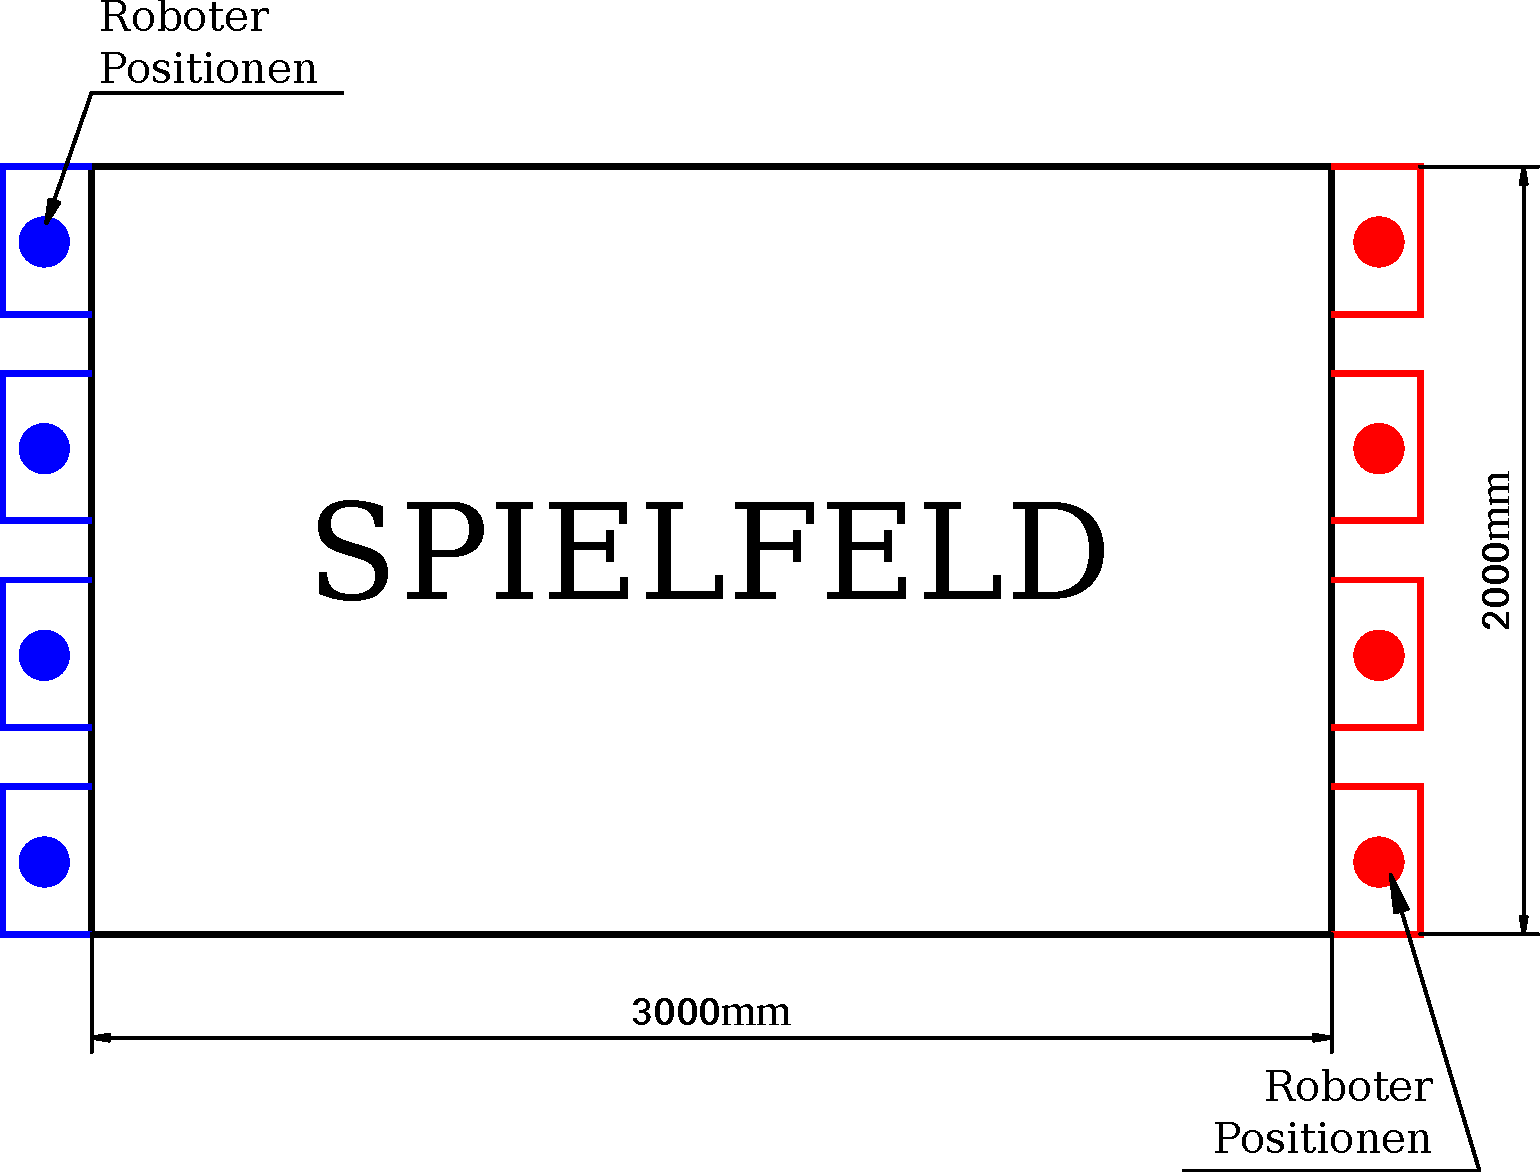
\includegraphics[width=0.8\textwidth]{Bilder/Spielfeld_2.pdf}
\end{center}
Es werden pro Gruppe 4 Roboter auf dem Spielfeld an ihre Startpositionen platziert.
Die Größe des Spielfeldes ist festgelegt.

%Alle Roboter, von beiden Teams, verbinden sich mit dem Server und übergeben diesem, dass Sie bereit sind.
%Sobald der Server das Startsignal gibt, fahren die Roboter mit einer Geschwindigkeit die $\frac{3}{4}$ der
%vollen Geschwindigkeit entspricht los.

Alle Roboter, von beiden Teams, verbinden sich mit dem Server und übergeben diesem, dass Sie bereit sind. Sobald der Server das Startsignal gibt, fahren alle Roboter los.

Dann versuchen sich die Roboter, der beiden Teams, gegenseitig zu fangen. Dazu muss einer der beiden Taster, welche am hinteren Ende des Roboters angebracht sind, betätigt werden.

%Befindet sich ein gegnerischer Roboter im Abstand X vor einem anderer Roboter, so wird die maximale Geschwindigkeit des hinteren Roboters freigeschaltet.

Wenn ein Roboter gefangen wurde, sendet dieser ein Signal an den Server und wird von diesem auf nicht Aktiv gesetzt.
Ist ein Roboter nicht Aktiv, so fährt dieser aus dem Spielfeld und verbleibt dort eine gewisse Zeit, bis er in's Spiel zurück kehrt.\\
\newline
\\
\textbf{Folgende Regeln wurden getroffen:}
\begin{itemize}
	\item Ein Roboter darf erst losfahren, wenn der Server das Startsignal gegeben hat
	\item Ein Roboter darf sich nicht um seine Achse drehen
	\item Ein Roboter darf nicht mit dem Rücken zur Wand stehen, da es so nicht möglich ist diesen zu fangen 
	%\item Erst ab einem Abstand X, darf die volle Geschwindigkeit zur Verfügung stehen
\end{itemize}
	\section{Zeitablauf}
\subsection{Gantt-Chart}
Ein Gantt-Diagramm oder auch Balkenplan ist ein Instrument des Projektmanagements, das die zeitliche Abfolge von Aktivitäten grafisch in Form von Balken auf einer Zeitachse darstellt.
\\\\
In den unteren Abbildungen sieht man einerseits die einzelnen Aktivitäten, Ressourcen und die Mitarbeiter die wir für unser Projekt "`Roboter-Fangen"' eingeplant haben, einmal als Liste und in einer grafischen Darstellung.

Außerdem kann man in der Liste erkennen, welche Aktivität welchen Vorgänger bzw. Nachfolger hat. Wo von es abhängig ist. 

Durch die grafische Darstellung ist es möglich frühzeitig Engpässe zu erkennen und das Projekt nötigen falls um zu strukturieren.
\\\\
Einige Aktivitäten haben wir der Übersichtlichkeit in Gruppen eingeteilt:\\\\
\begin{tabular}{p{0.5\textwidth}p{0.5\textwidth}}
	\textbf{Gruppen:} & \textbf{Meilensteine:}\\
	\begin{itemize}
		\item Planung
		\item Programmierung-Teil 1
		\begin{itemize}
			\item Simple KI
		\end{itemize}
		\item Programmierung-Teil 2
		\item Dokumentation
	\end{itemize} & 
	\begin{itemize}
		\item M0: Start
		\item M1: Planung abgeschlossen
		\item M2: Erste Implementierung
		\item M3: Kurzpräsentation
		\item M4: Programmierung abgeschlossen
		\item M5: Endpräsentation
		\item M6: Dokumentation abgeschlossen
	\end{itemize}\\
\end{tabular}
\\
\begin{center}
		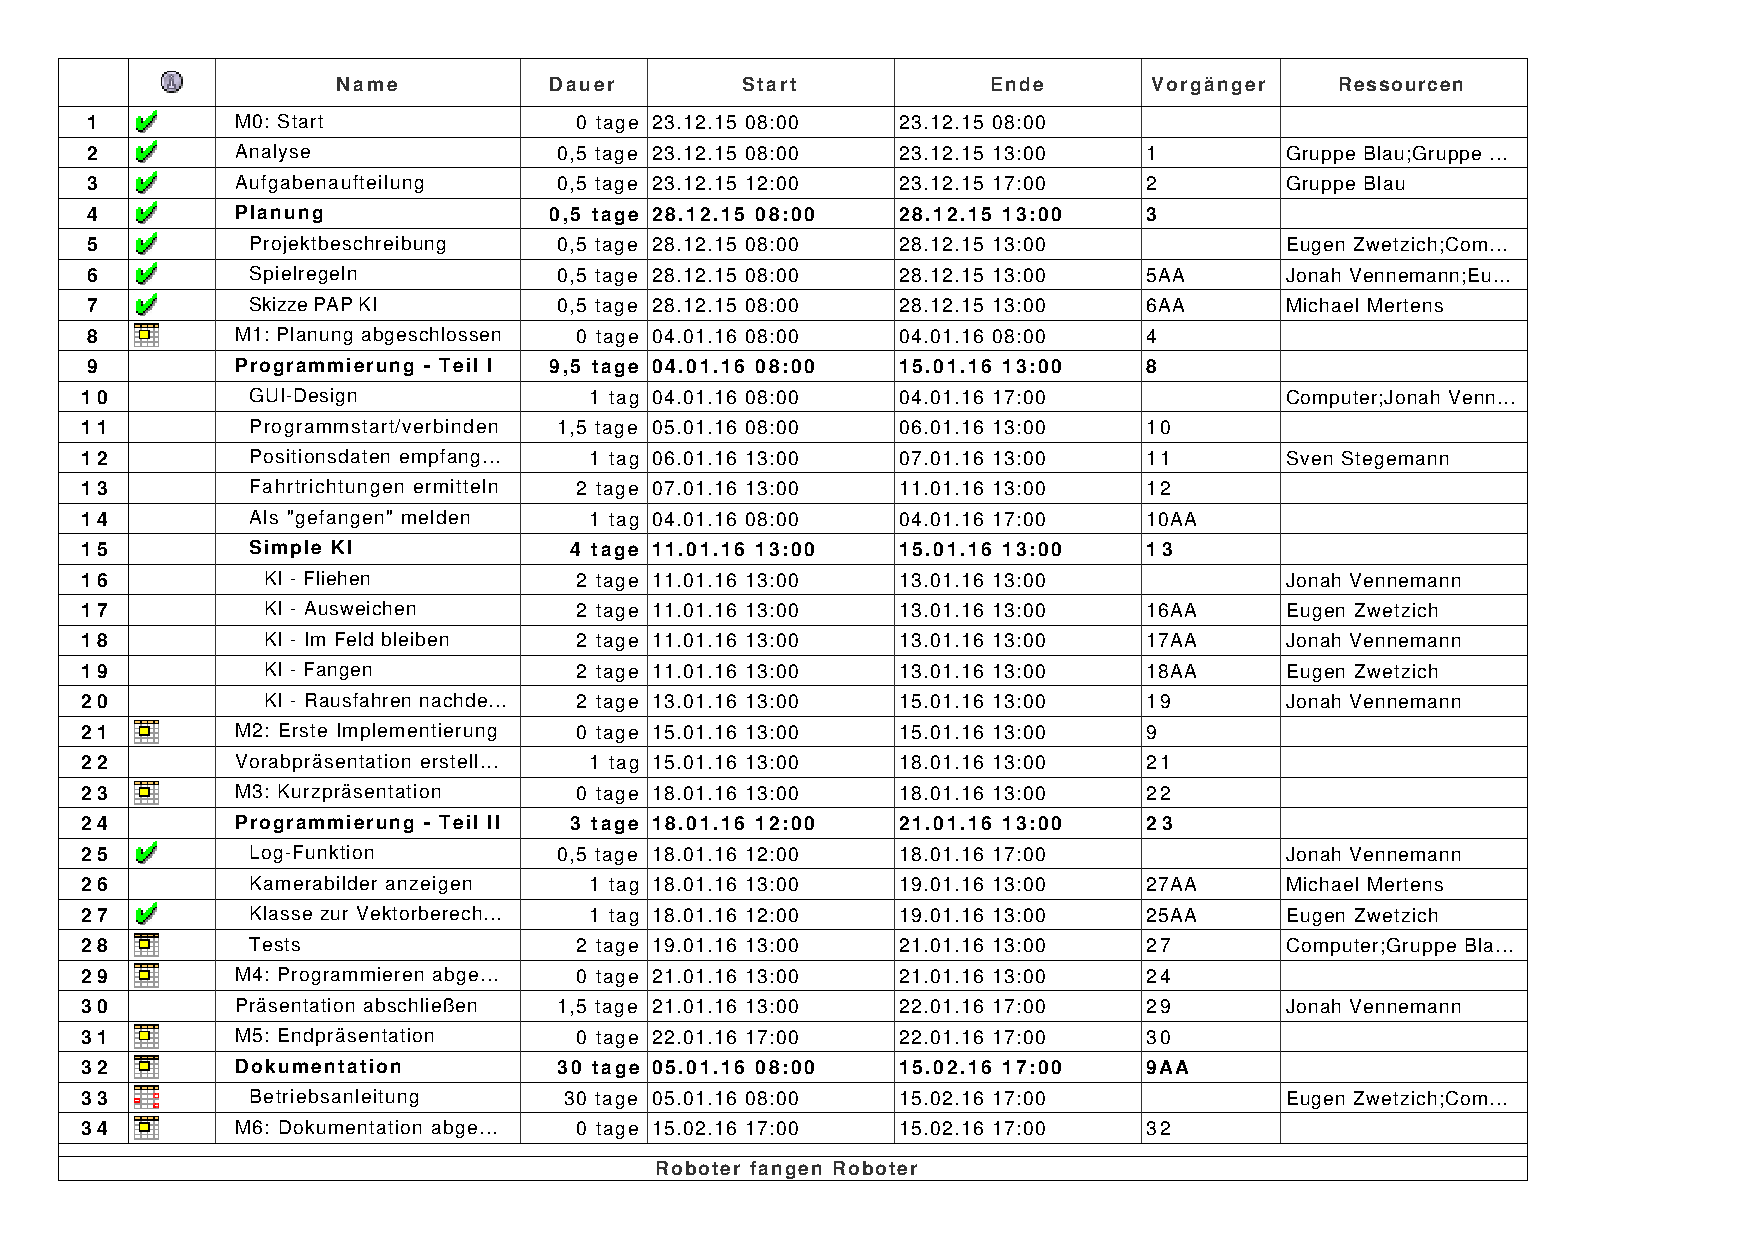
\includegraphics[width=0.8\textwidth]{Bilder/GanttDiagramm_[Page1].pdf}
		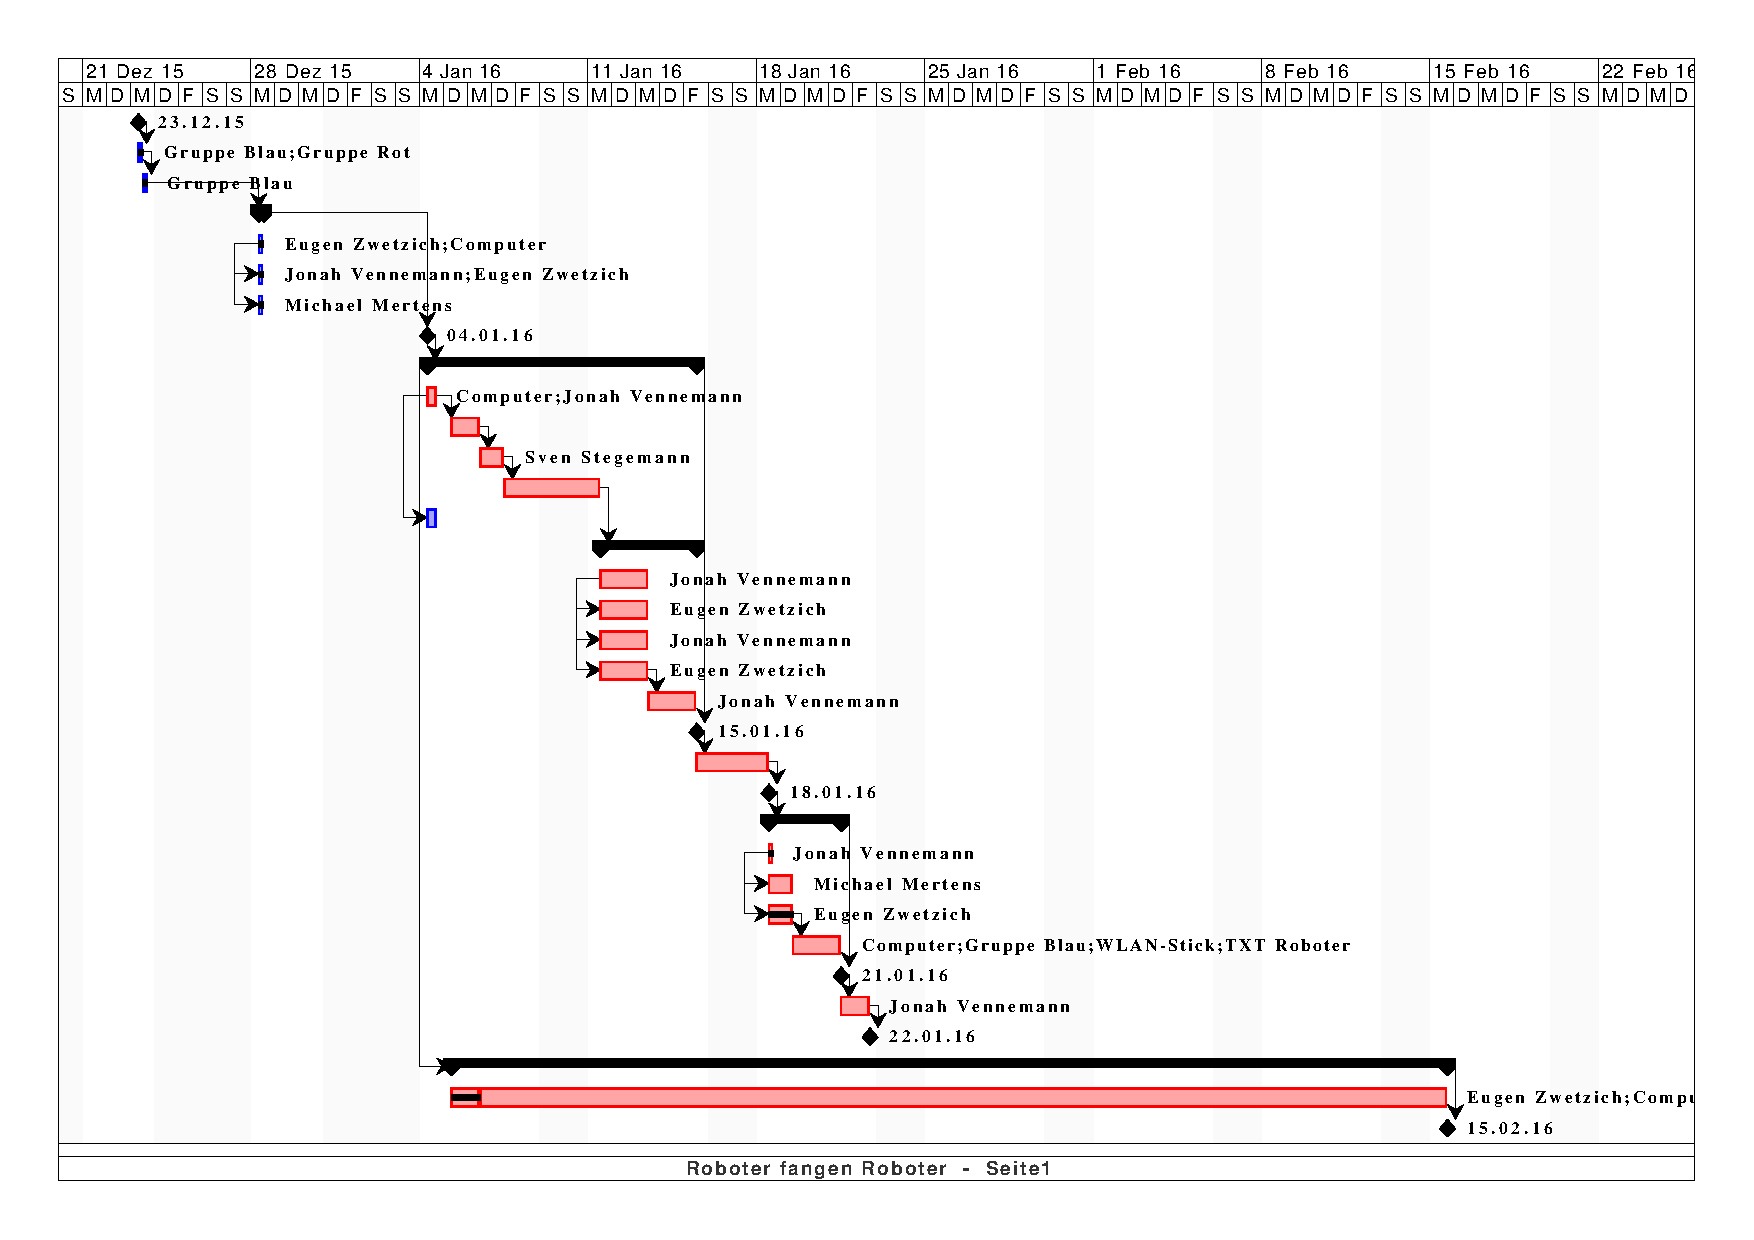
\includegraphics[width=0.8\textwidth]{Bilder/GanttDiagramm_[Page2].pdf}
		\captionof{figure}{Gantt-Chart v1.0}
\end{center}
\newpage
Aufgrund von Komplikationen mit den Roboter Klassen, mit dem Voranstreiten der Programmierung des Servers und der Komplexität der Programmierung der KI mussten wir die Planung des Projektes umstrukturieren.

Wir haben die Aktivitäten für die Benutzeroberfläche, das Ereignisprotokoll und die Vektorberechnung in den Programmierung-Teil 1 vorgezogen.

Erst im 2. Teil der Programmierung fingen wir mit der Programmierung der KI und der Kommunikation mit dem Server an.
\\\\
\textbf{Gruppen:} 
\begin{itemize}
	\item Planung
	\item Programmierung-Teil 1
	\item Programmierung-Teil 2
	\begin{itemize}
		\item Simple KI
	\end{itemize}
	\item Server-Team\\
\end{itemize} 
\textbf{Meilensteine:}
\begin{description}
	\item[M1: Planung abgeschlossen] Es muss die Projektbeschreibung, eine Skizze für die KI und ein Spielablauf fertig sein.
	\item[M2: Kurzpräsentation] Eine Präsentation über die zeitliche Planung und über die Aufwandsschätzung
	\item[M3: Programmierung abgeschlossen] Es muss die ganze Programmierung(Vektorberechnung, Künstliche Intelligenz, Benutzeroberfläche) der Software abgeschlossen sein. 
	\item[M4: Endpräsentation] Eine Abschlusspräsentation vom Projekt mit einer Vorführung des Spiels
	\item[M4: Dokumentation abgeschlossen] Abgabe der Dokumentation in ausgedruckter und digitaler Form
\end{description}

\begin{center}
	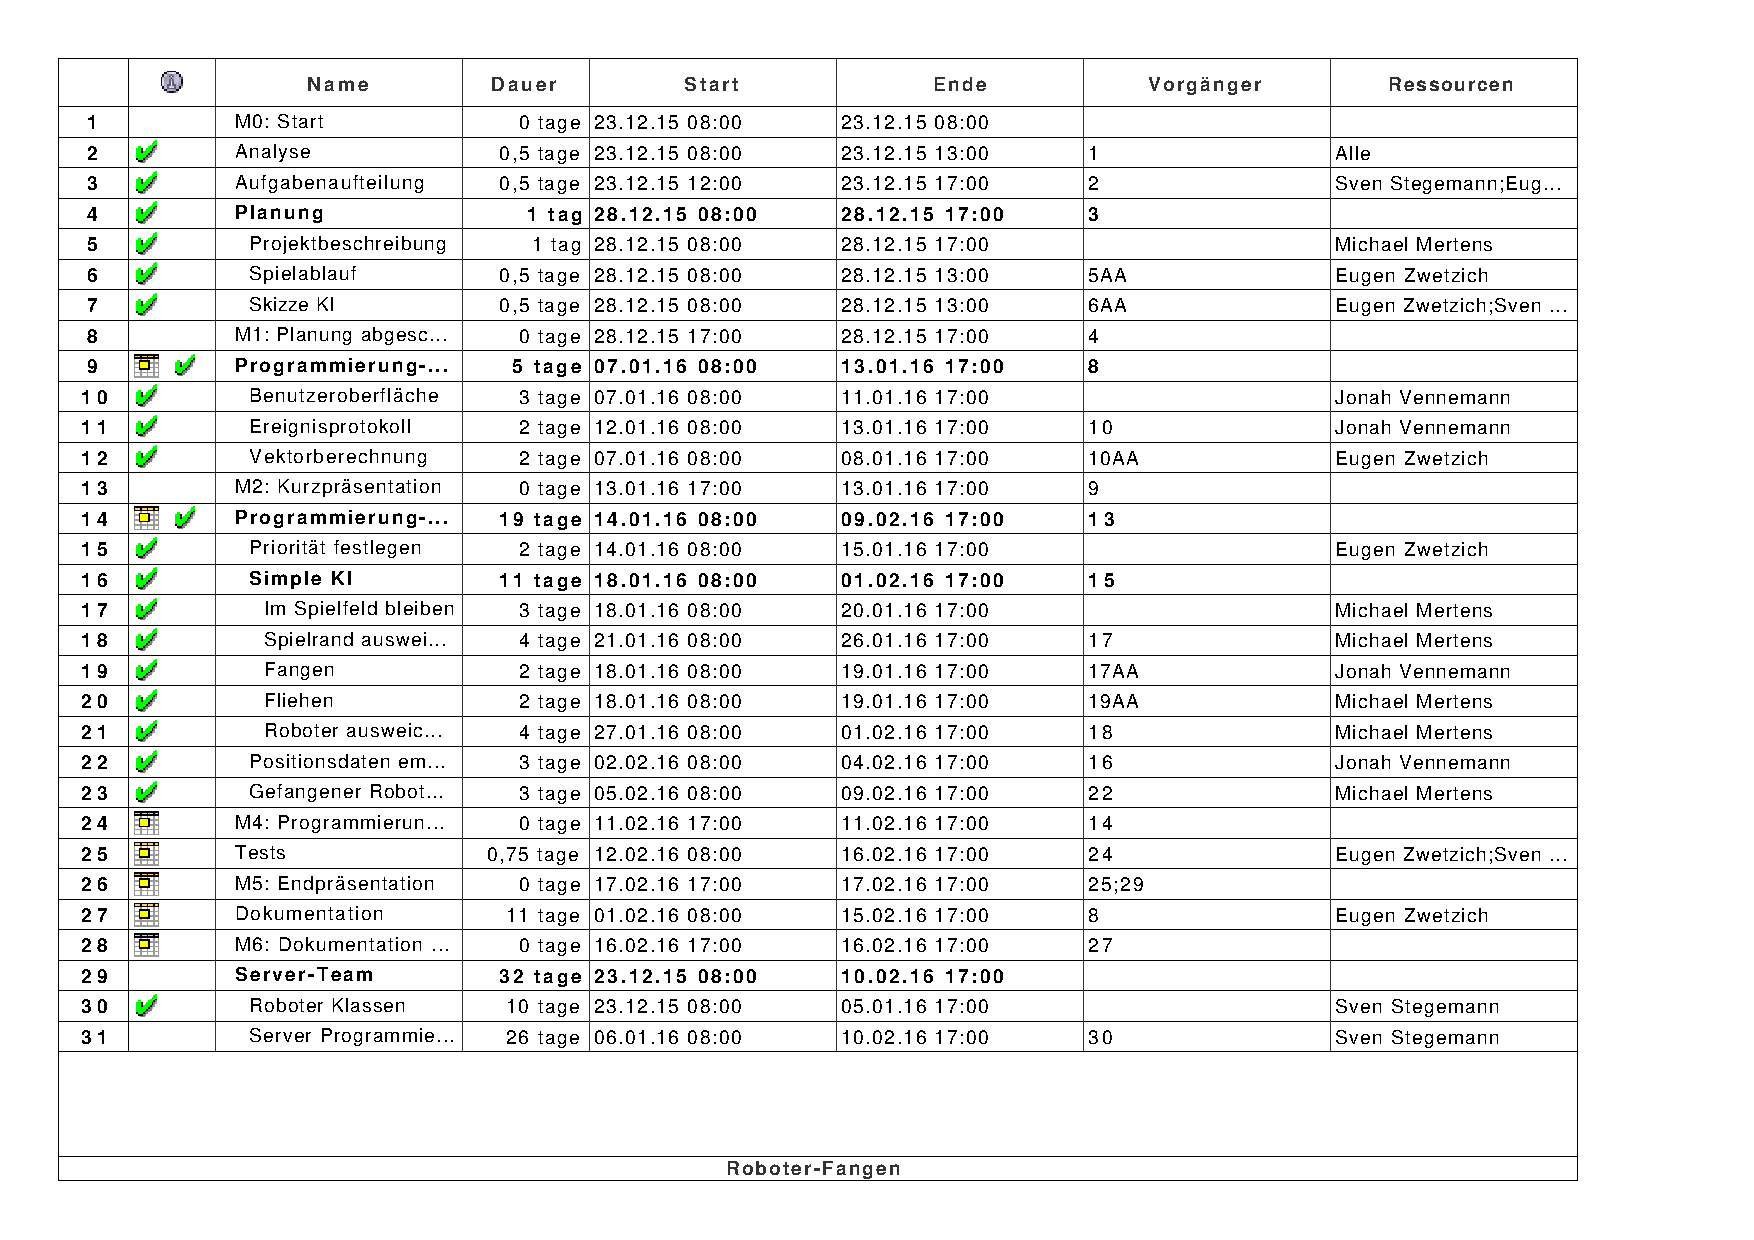
\includegraphics[width=0.8\textwidth]{Bilder/Roboter-Fangen_Liste.pdf}
	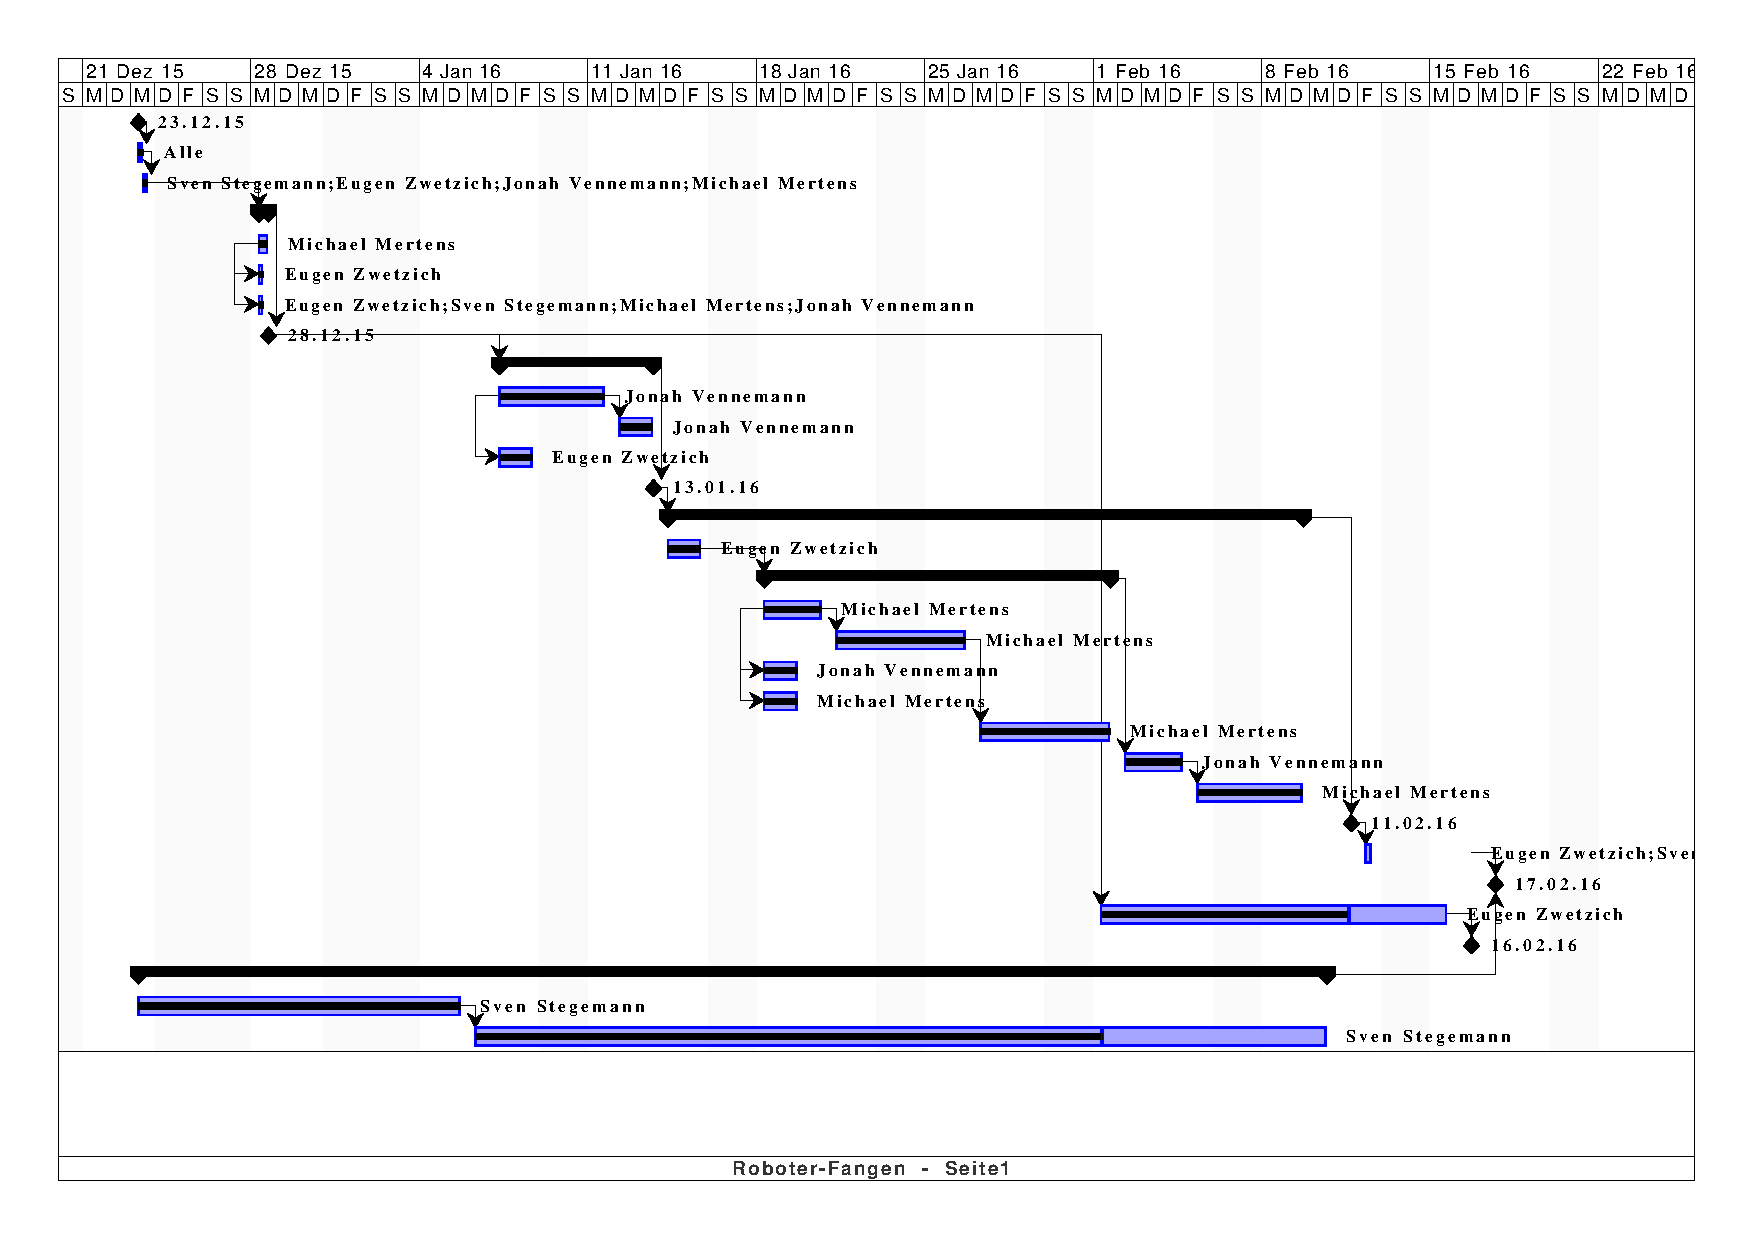
\includegraphics[width=0.8\textwidth]{Bilder/Roboter-Fangen_Grafik.pdf}
	\captionof{figure}{Gantt-Chart v2.0}
\end{center}
\newpage
	\section{Aufwandsschätzung}
Um den Aufwand unseres IT-Projektes abschätzen zu können, haben wir die Methode Function-Point benutzt.

Das Function-Point-Verfahren(auch -Analyse oder -Methode, kurz: FPA) dient der Bewertung des fachlich-funktionalen Umfangs eines Informationstechnischen Systems.\\
\newline
Die Durchführung des Verfahrens verläuft in 5 Schritten:
\begin{enumerate}
	\item Analyse der Komponenten und Kategorisierung ihrer Funktionalitäten
	\item Bewertung der verschiedenen Funktionskategorien
	\item Einbeziehung besonderer Einflussfaktoren
	\item Ermittlung der sog. Total Function Points(TFP)
	\item Ableitung des zu erwartenden Entwicklungsaufwandes
\end{enumerate}
\vspace{0.2cm}
\paragraph{1. Schritt}
\begin{itemize}
	\item Eingabedaten
	\begin{itemize}
		\item GUI
		\item Programmstart
	\end{itemize}
	\item Ausgabedaten
	\begin{itemize}
		\item Ereignisprotokolldatei
		\item Kamerabild
		\item Steuerbefehle senden
	\end{itemize}
	\item projektbez. Datenbestände
	\begin{itemize}
		\item Fahrtrichtung
		\item Fangen
		\item Fliehen
		\item Ausweichen
		\item Im Feld bleiben
		\item Rausfahren nach dem Fangen
		\item Vektorberechnung
	\end{itemize}
	\item externe Datenbestände
	\begin{itemize}
		\item Positionsdaten
		\item Mitteilung gefangen
		\item Roboter aktiv?
	\end{itemize}
\end{itemize}

\newpage
\begin{landscape}
	\paragraph{2. Schritt}
	\begin{center}
		\begin{tabular}{|l|ccc|ccc|ccc|}
			\hline
			\multirow{2}{*}{Funktionskategorie} & \multicolumn{3}{c|}{Anzahl der Funktionen} & \multicolumn{3}{c|}{Faktoren der Funktionen} & \multicolumn{3}{c|}{Funktionspunkte}\\
			& Einfach & Mittel & Komplex & Einfach & Mittel & Komplex & Einfach & Mittel & Komplex\\
			\hline
			Eingabedaten & 1 & 1 & 0 & 3 & 4 & 6 & 3 & 4 & 0\\
			Ausgabedaten & 1 & 2 & 0 & 4 & 5 & 7 & 4 & 10 & 0\\
			Projektbez. Datenbestände & 1 & 3 & 3 & 7 & 10 & 15 & 7 & 30 & 45\\
			Externe Datenbestände & 3 & 0 & 0 & 5 & 7 & 10 & 15 & 0 & 0\\
			\hline
			\multicolumn{10}{c}{}\\
			\cline{8-10}
			\multicolumn{7}{c}{} & \multicolumn{2}{|l|}{{\bf Summe S$1$:}} & {\bf $118$}\\
			\cline{8-10}			
		\end{tabular}
	\end{center}
	\vspace{0.2cm}
	\begin{minipage}{0.7\textwidth}
		\paragraph{3. Schritt}
		\begin{center}
			\begin{tabular}{|c|l|c|}
				\hline
				Nr & Einflussfaktoren & Gewichte\\
				\hline
				1 & Schwierigkeit und Komplexität der Rechenoperatoren (Faktor 2) & 2\\
				2 & Schwierigkeit und Komplexität der Ablauflogik & 5\\
				3 & Umfang der Ausnahmeregelung (Faktor 2) & 6\\
				4 & Verflechtungen mit anderen IT-Systemen & 3\\
				5 & dezentrale Verarbeitung und Datenhaltung & 0\\
				6 & erforderliche Maßnahmen der IT Sicherheit & 0\\
				7 & angestrebte Rechengeschwindigkeit & 1\\
				8 & Konvertierung der Datenbeständen & 0\\
				9 & Benutzer- und Änderungsfreundlichkeit & 1\\
				10 & Wiederverwendbarkeit von Komponenten (bspw. Klassen) & 1\\
				\hline
				\multicolumn{3}{c}{}\\
				\cline{2-3}
			    \multicolumn{1}{c}{} & \multicolumn{1}{|l|}{{\bf Summe S$2$:}} & $19$\\
				\cline{2-3} 
			\end{tabular}
		\end{center}
	\end{minipage}
\end{landscape}

\paragraph{4. Schritt}
\begin{align*}
	\text{TFP\footnotemark} &= \text{S}1 \cdot \text{S}3\\
			   &= \text{S}1 \cdot \left(0{,}7 + \frac{\text{S}2}{100}\right)\\
			   &= 118 \cdot \left( 0{,}7 + \frac{19}{100}\right)\\
	\text{TFP} &= 105{,}02\\
\end{align*}\footnotetext{TFP=Total Function Points}
\paragraph{5. Schritt}
\[\text{PM\footnotemark} = 0{,}08 \cdot \text{TFP}-7 \leq 1000\text{TFP} > \text{PM} = 0{,}08 \cdot \text{TFP}-108\]
\begin{align*}
	\text{PM} &= 0{,}08 \cdot \text{TFP} - 7 \\
			  &= 0{,}08 \cdot 105{,}02 -7\\
	\text{PM} &= 1{,}4016\\
	\\
	\text{PM} &= 672{,}77 \text{h}\\
	\\
	\text{3 Personen} &= 224{,}256\text{h pro Person}\\
	\text{4 Personen} &= 168{,}192\text{h pro Person}\\
\end{align*}\footnotetext{Personenmonate(PM) = 20 Arbeitstage}

$\Rightarrow$ Bei einem 4 starken Team benötigen wir ca. 170h pro Person.

	\section{GitHub}
GitHub ist ein webbasierter Online-Dienst, für die Versionsverwaltungssoftware Git.

In GitHub haben wir unser Projekt 
\begin{center}
	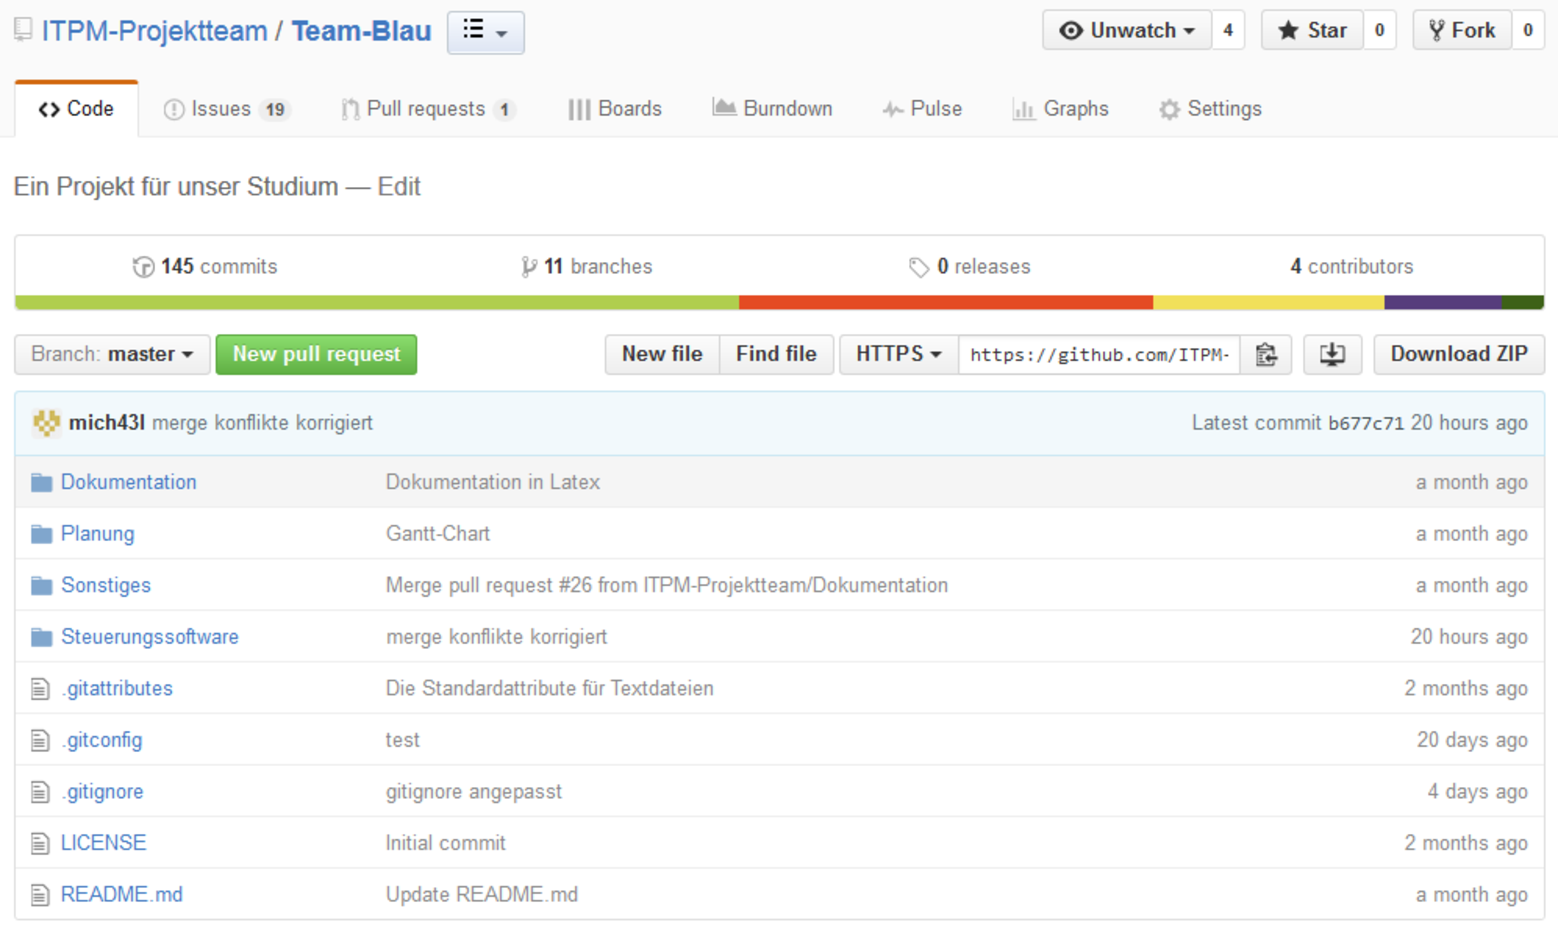
\includegraphics[scale=0.5]{Bilder/Github.pdf}
\end{center}


	
	\subsection{ZenHub}
ZenHub ist eine Projektmanagement-Erweiterung für GitHub.
\\
ZenHub haben wir dafür benutzt, um die Programmierung des Projektes in Hauptkategorien auf zu teilen.
Diesen Kategorien haben wir Mitarbeiter zu geteilt, sowie die eventuell benötigte Dauer, für die Erstellung der Punkte vergeben.
\\\\
ZenHub unterteilt sich in:
\begin{itemize}
	\item New Issues(Neue Hauptpunkte)
	\item Ice-Box(Eingefrorene Punkte)
	\item Backlog(Arbeitsrückstand)
	\item To Do(Muss gemacht werden)
	\item In Progress(In Bearbeitung)
	\item Done/Review(Fertig/Überprüfung) 
\end{itemize}
\begin{landscape}
	\begin{center}
		\begin{tabulary}{1\textwidth}{cc}
			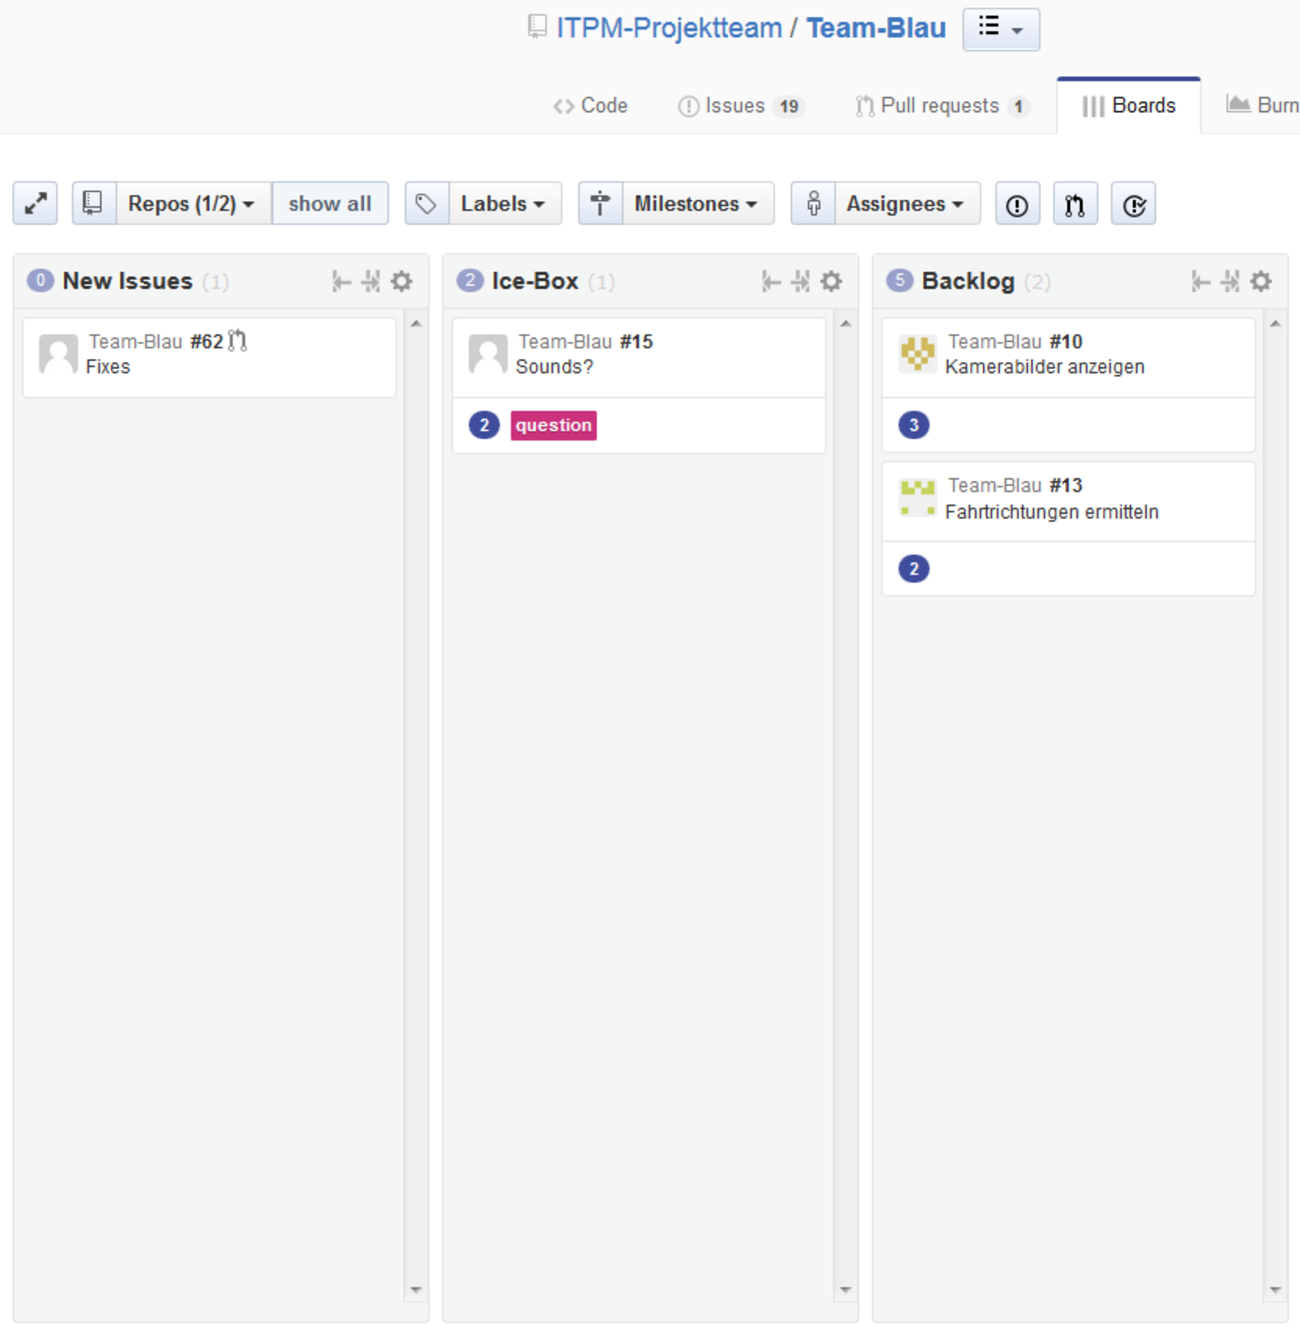
\includegraphics[scale=0.5]{Bilder/ZenHub1.pdf} 
			&
			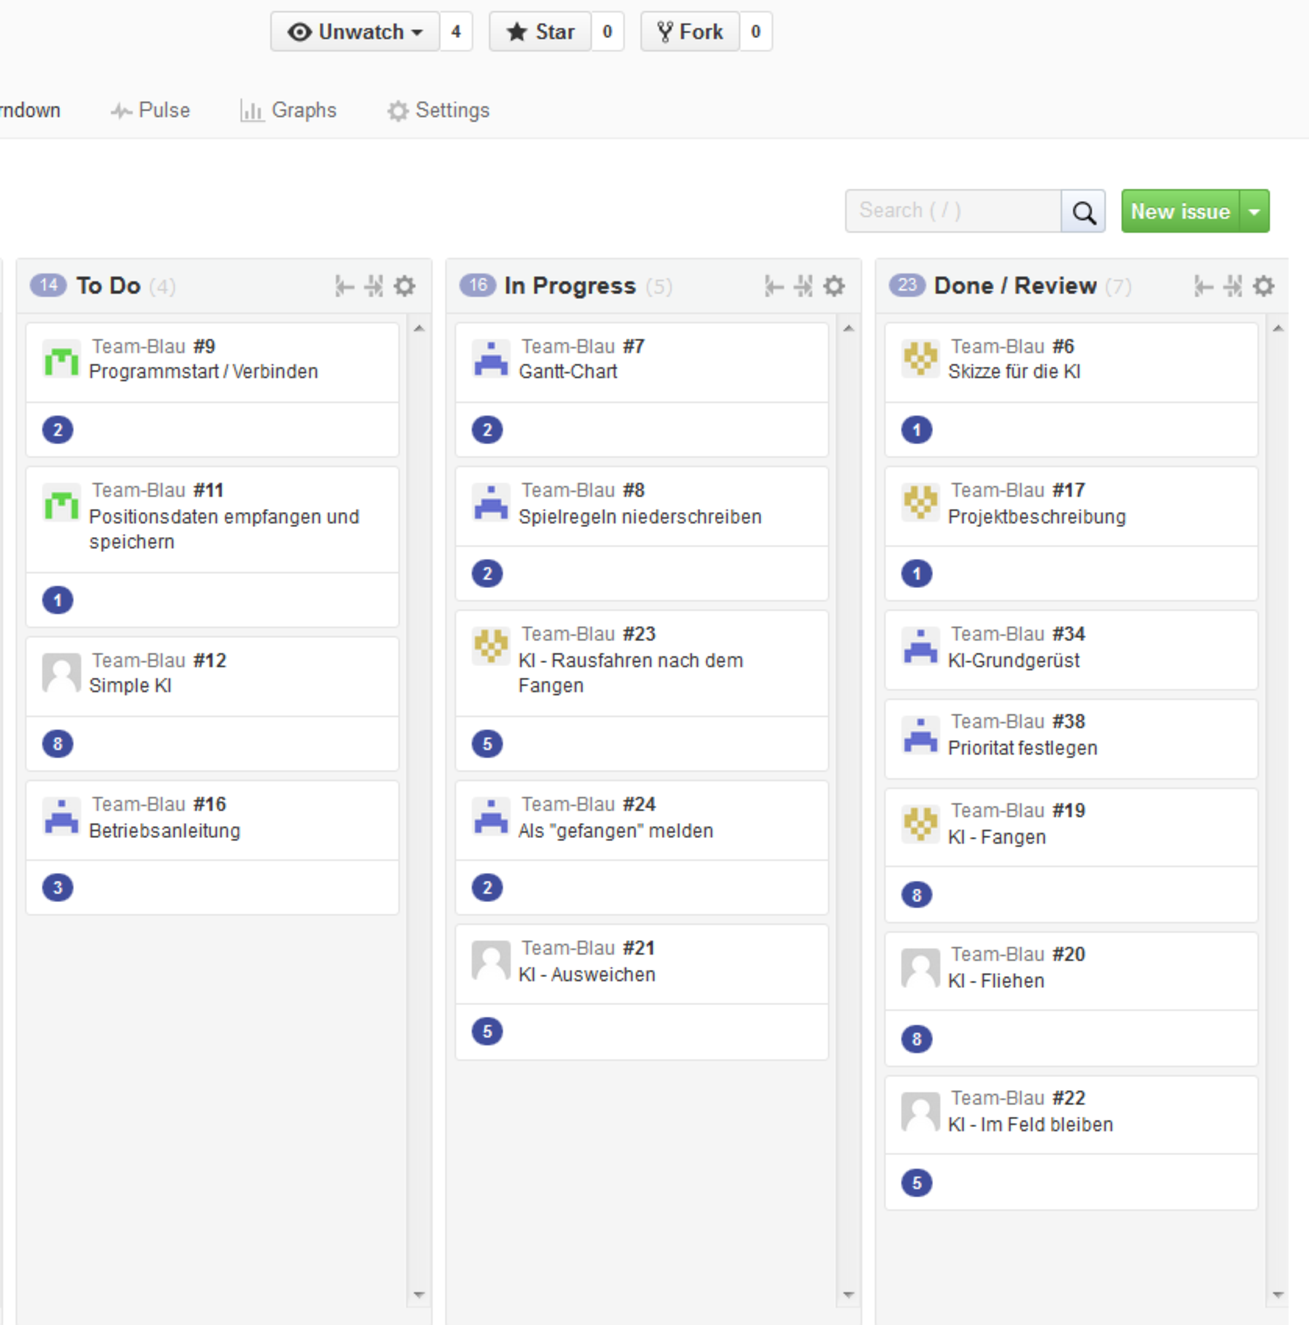
\includegraphics[scale=0.5]{Bilder/ZenHub2.pdf}\\
		\end{tabulary}
		\captionof{figure}{Auflistung der Punkte in ZenHub}
	\end{center}
\end{landscape}
	\section{Systemaufbau}
\begin{center}
	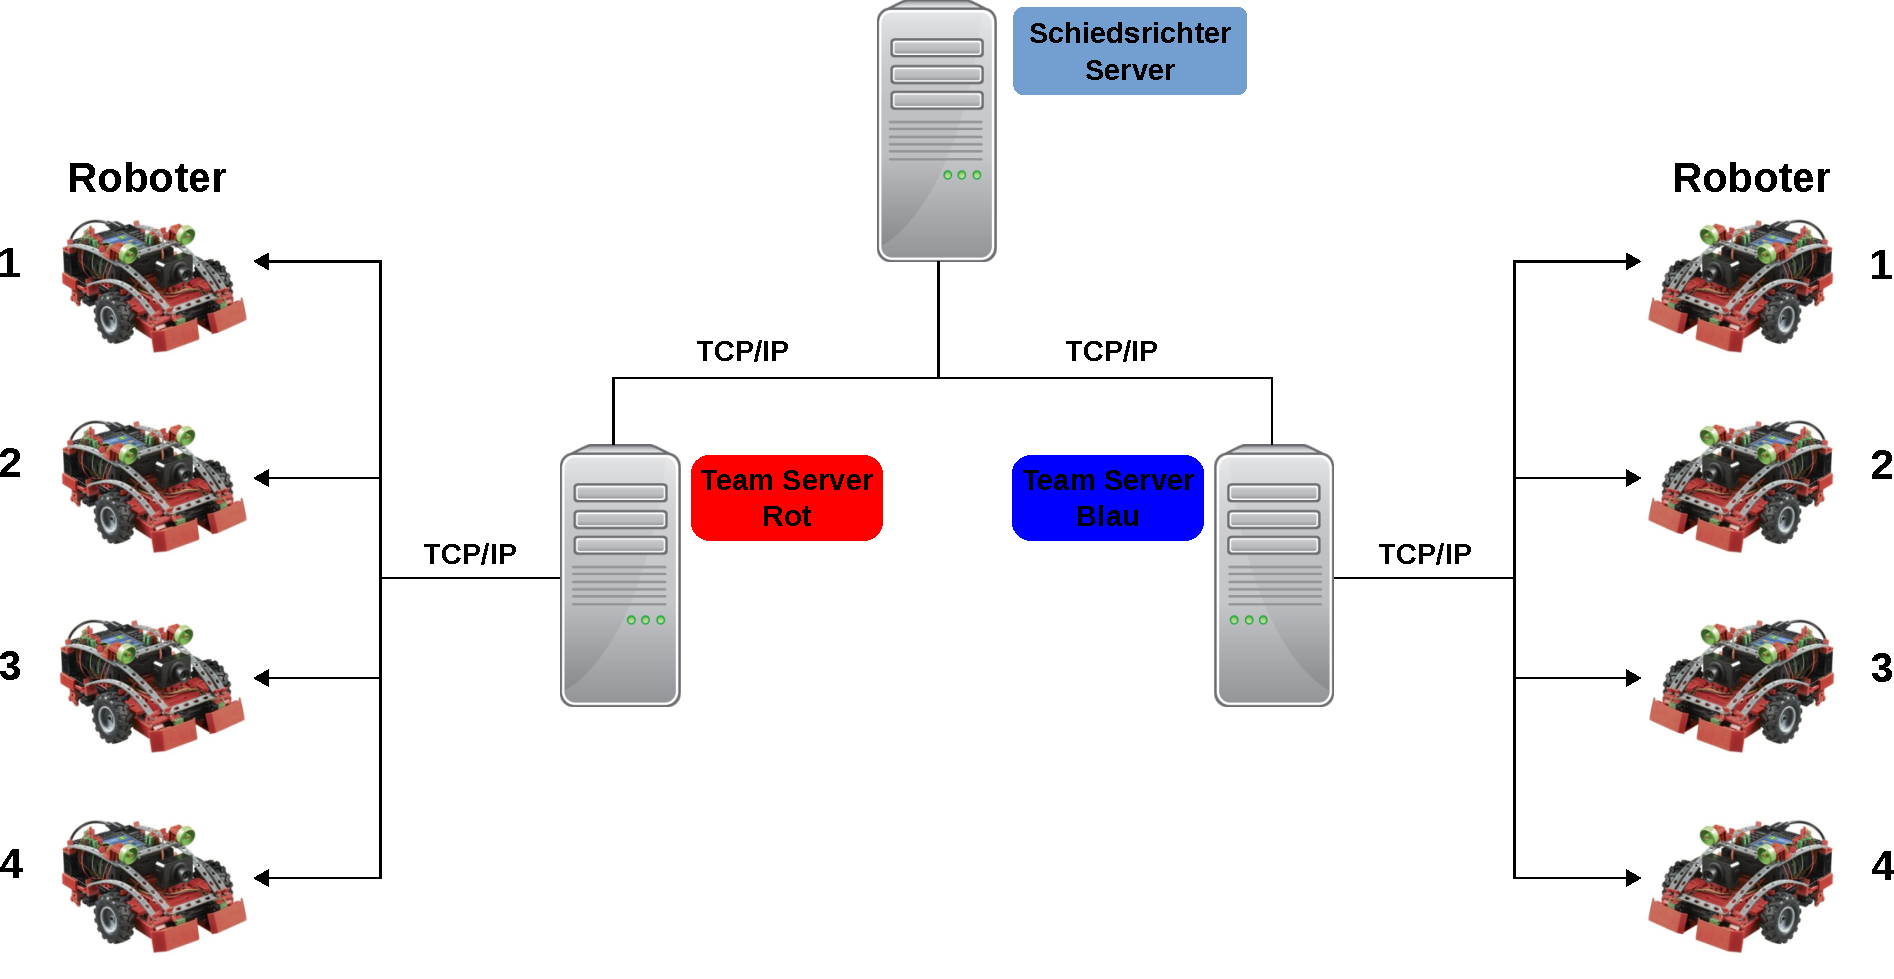
\includegraphics[scale=0.5]{Bilder/Systemaufbau.pdf}
\end{center}
Der Systemaufbau des Projekts stellt sich wie folgt dar:
\newline
Ein zentraler Schiedsrichter-Server überwacht das Spielfeld der Roboter mithilfe einer Kamera. Anhand der Kamerabilder werden Positionsdaten der Roboter bestimmt. Des weiteren überwacht der Server den Status der Roboter, d.h. es wird überprüft ob diese gefangen wurden.

Die Positionsdaten werden mittels einer TCP/IP-Verbindung an die jeweiligen Team-Server gesendet. Diese werten die Daten aus und ermitteln die Fahrtrichtungen für jeden Roboter eines Teams. Die Befehle werden wieder mithilfe einer TCP/IP-Verbindung an die Roboter übermittelt.



	\section{Programmierung}
\subsection{Programmablaufplan}
\vspace{1cm}
\begin{center}
	\tikzstyle{startstop} = [rectangle, rounded corners, minimum width=3cm, minimum height=1cm,text centered, draw=black, fill=red!30]
	\tikzstyle{io} = [trapezium, trapezium left angle=70, trapezium right angle=110, minimum width=3cm, minimum height=1cm, text centered, draw=black, fill=blue!30]
	\tikzstyle{process} = [rectangle, minimum width=3cm, minimum height=1cm, text centered, text width=3cm, draw=black, fill=orange!30]
	\tikzstyle{decision} = [diamond, minimum width=1cm, minimum height=1cm, text centered, text width=3cm, draw=black, fill=green!30]
	\tikzstyle{arrow} = [thick,->,>=stealth]
	\begin{tikzpicture}[node distance=2cm]
		\node (start) [startstop] {Start};
		\node (pro1) [process,below of=start] {Vordefinierter Anfangsweg};
		\node (in1) [io,below of=pro1] {Eingabedaten verarbeiten};
		\node (dec1) [decision,below of=in1,yshift=-1cm] {Roboter aktiv?};
		\node (dec2) [decision,below of=dec1,xshift=3.5cm,yshift=-2cm] {Priorität festlegen};
		\node (pro2) [process,below of=dec1,xshift=-4cm,yshift=-2cm] {Herausfahrvektor berechnen};
		\node (pro3) [process,below of=dec2,xshift=-4cm,yshift=-1.5cm] {Verfolgungsvektor berechnen};
		\node (pro4) [process,below of=dec2,xshift=4cm,yshift=-1.5cm] {Fliehvektor berechnen};
		\node (pro5) [process,below of=pro3,xshift=4cm,yshift=-1cm] {Vektor anpassen};
		\node (in2) [io,below of=pro5] {Befehle senden};
		
		\draw [arrow] (start) -- (pro1);
		\draw [arrow] (pro1) -- (in1);
		\draw [arrow] (in1) -- (dec1);
		\draw [arrow] (dec1) -| node[anchor=south] {ja} (dec2);
		\draw [arrow] (dec1) -| node[anchor=south] {nein} (pro2);
		\draw [arrow] (dec2) -| node[anchor=south] {fangen} (pro3);
		\draw [arrow] (dec2) -| node[anchor=south] {fliehen} (pro4);
		\draw [arrow] (pro2) |- (pro5);
		\draw [arrow] (pro3) -| (pro5);
		\draw [arrow] (pro4) -| (pro5);
		\draw [arrow] (pro5) -- (in2);
		\draw [arrow] (in2) -| (10.5, -8) |- (0,-3);
	\end{tikzpicture}
\end{center}
\newpage

\subsection{Klassendiagramm}

\begin{center}
	\resizebox{\textwidth}{!}{
		\begin{tikzpicture}[show background grid]
		\begin{class}[text width=5cm]{THauptforumular}{-5,1.85}
		\attribute{+ Anz\_Roboter: Integer}
		\attribute{+ B\_Verbinden: TButton}
		\attribute{+ CB\_Bereit: TCheckBox}
		\attribute{+ G\_Steuerung: TGroupBox}
		\attribute{+ I\_MiniMap: TImage}
		\attribute{+ I\_Roboter1: TImage}
		\attribute{+ I\_Roboter2: TImage}
		\attribute{+ I\_Roboter3: TImage}
		\attribute{+ I\_Roboter4: TImage}
		\attribute{+ IP\_Adressen: Array of String}
		\attribute{+ IPConfig: Textfile}2
		\attribute{+ Label1: TLabel}
		\attribute{+ M\_Log: TMemo}
		\attribute{+ Port: Integer}
		\attribute{+ Server\_IP: String}
		\operation{+ B\_VerbindenClick}
		\operation{+ CB\_BereitClick}
		\operation{+ FormCreate}
		\operation{+ KamerabilderAnzeigen}
		\operation{+ Log\_Schreiben}
		\operation{+ Visualisieren}
		\end{class}
		
		\begin{class}[text width=6cm]{TKI}{3,2}
		\attribute{- Client: TServerVerbindung}
		\attribute{- Formular: THauptformular}
		\attribute{- Roboter: Array of TTXTMobilRoboter}
		\attribute{- RoboterDaten: Array[TTeam] of Array of TRoboterDaten}
		\attribute{- Spielfeld: TVektor}
		\attribute{- ZeitLetzterFrames: TQueue<TDateTime>}
		\operation{+ Anmelden}
		\operation{+ Init}
		\operation{+ Steuern}
		\operation{- FangvektorBerechnen: TVektor}
		\operation{- FliehvektorBerechnen: TVektor}
		\operation{- GeschwindigkeitenBerechnen}
		\operation{- PrioritaetFestlegen: TAktion}
		\operation{- RandAusweichvektorBerechnen: TVektor}
		\operation{- RausfahrvektorBerechnen: TVektor}
		\operation{- RoboterAusweichvektorBerechnen: TVektor}
		\operation{- ServerdatenEmpfangen: Boolean}
		\operation{- SteuerbefehlSenden}
		\end{class}
		
		\begin{record}[text width=5.3cm]{TVektor}{11,-0.6}
		\attribute{+ x: Double}
		\attribute{+ y: Double}
		\operation{+ Betrag: Double}
		\operation{+ Drehen: TVektor}
		\operation{+ operator Add: TVektor}
		\operation{+ operator Equal: Boolean}
		\operation{+ operator Multiply: TVektor}
		\operation{+ operator Multiply: TVektor}
		\operation{+ operator Subtract: TVektor}
		\operation{+ Winkel: TVektor}
		\operation{+ Winkel: TVektor}
		\end{record}
		
		\begin{record}[text width=7cm]{TRoboterDaten}{11,-9}
		\attribute{+ Aktiv: Boolean}
		\attribute{+ Geschwindigkeit: TVektor}
		\attribute{+ Position: TVektor}
		\attribute{+ Positionsverlauf: TQueue<TVektor>}
		\end{record}
		
		\begin{class}[text width=6cm]{TTXTMobilRoboter}{3,-12}
		\attribute{+ ID: Integer}
		\attribute{+ kamThread: TKameraThread}
		\attribute{+ nwThread: TNetzwerkThread}
		\operation{+ BewegenAlle}
		\operation{+ BewegenAlleBis}
		\operation{+ BewegenEiner}
		\operation{+ BewegenEinerBis}
		\operation{+ Create}
		\operation{+ Destroy}
		\operation{+ Ende}
		\operation{+ HoleID: Integer}
		\operation{+ Start}
		\operation{+ ZielErreicht: Boolean}
		\end{class}
		
		\begin{class}[text width=5cm]{TNetzwerkThread}{11,-13.95}
		\attribute{callback: TCallback}
		\attribute{delay: Integer}
		\attribute{roboter: TTXTMobilRoboter}
		\operation{+ Create}
		\operation{+ Execute}
		\end{class}
		
		\begin{class}[text width=5cm]{TKameraThread}{-5,-13.95}
		\attribute{callback: TCallback}
		\attribute{delay: Integer}
		\attribute{roboter: TTXTMobilRoboter}
		\operation{+ Create}
		\operation{+ Execute}
		\end{class}
		
		\association{TKI}{}{}{THauptforumular}{}{}
		\composition{TKI}{}{}{TVektor}{}{}
		\composition{TKI}{}{}{TRoboterDaten}{}{}
		\association{TTXTMobilRoboter}{}{}{TKI}{}{}
		\aggregation{TTXTMobilRoboter}{}{}{TNetzwerkThread}{}{}
		\aggregation{TTXTMobilRoboter}{}{}{TKameraThread}{}{}
		\end{tikzpicture}
	}
\end{center}

\subsection{Hauptformular}
\begin{center}
	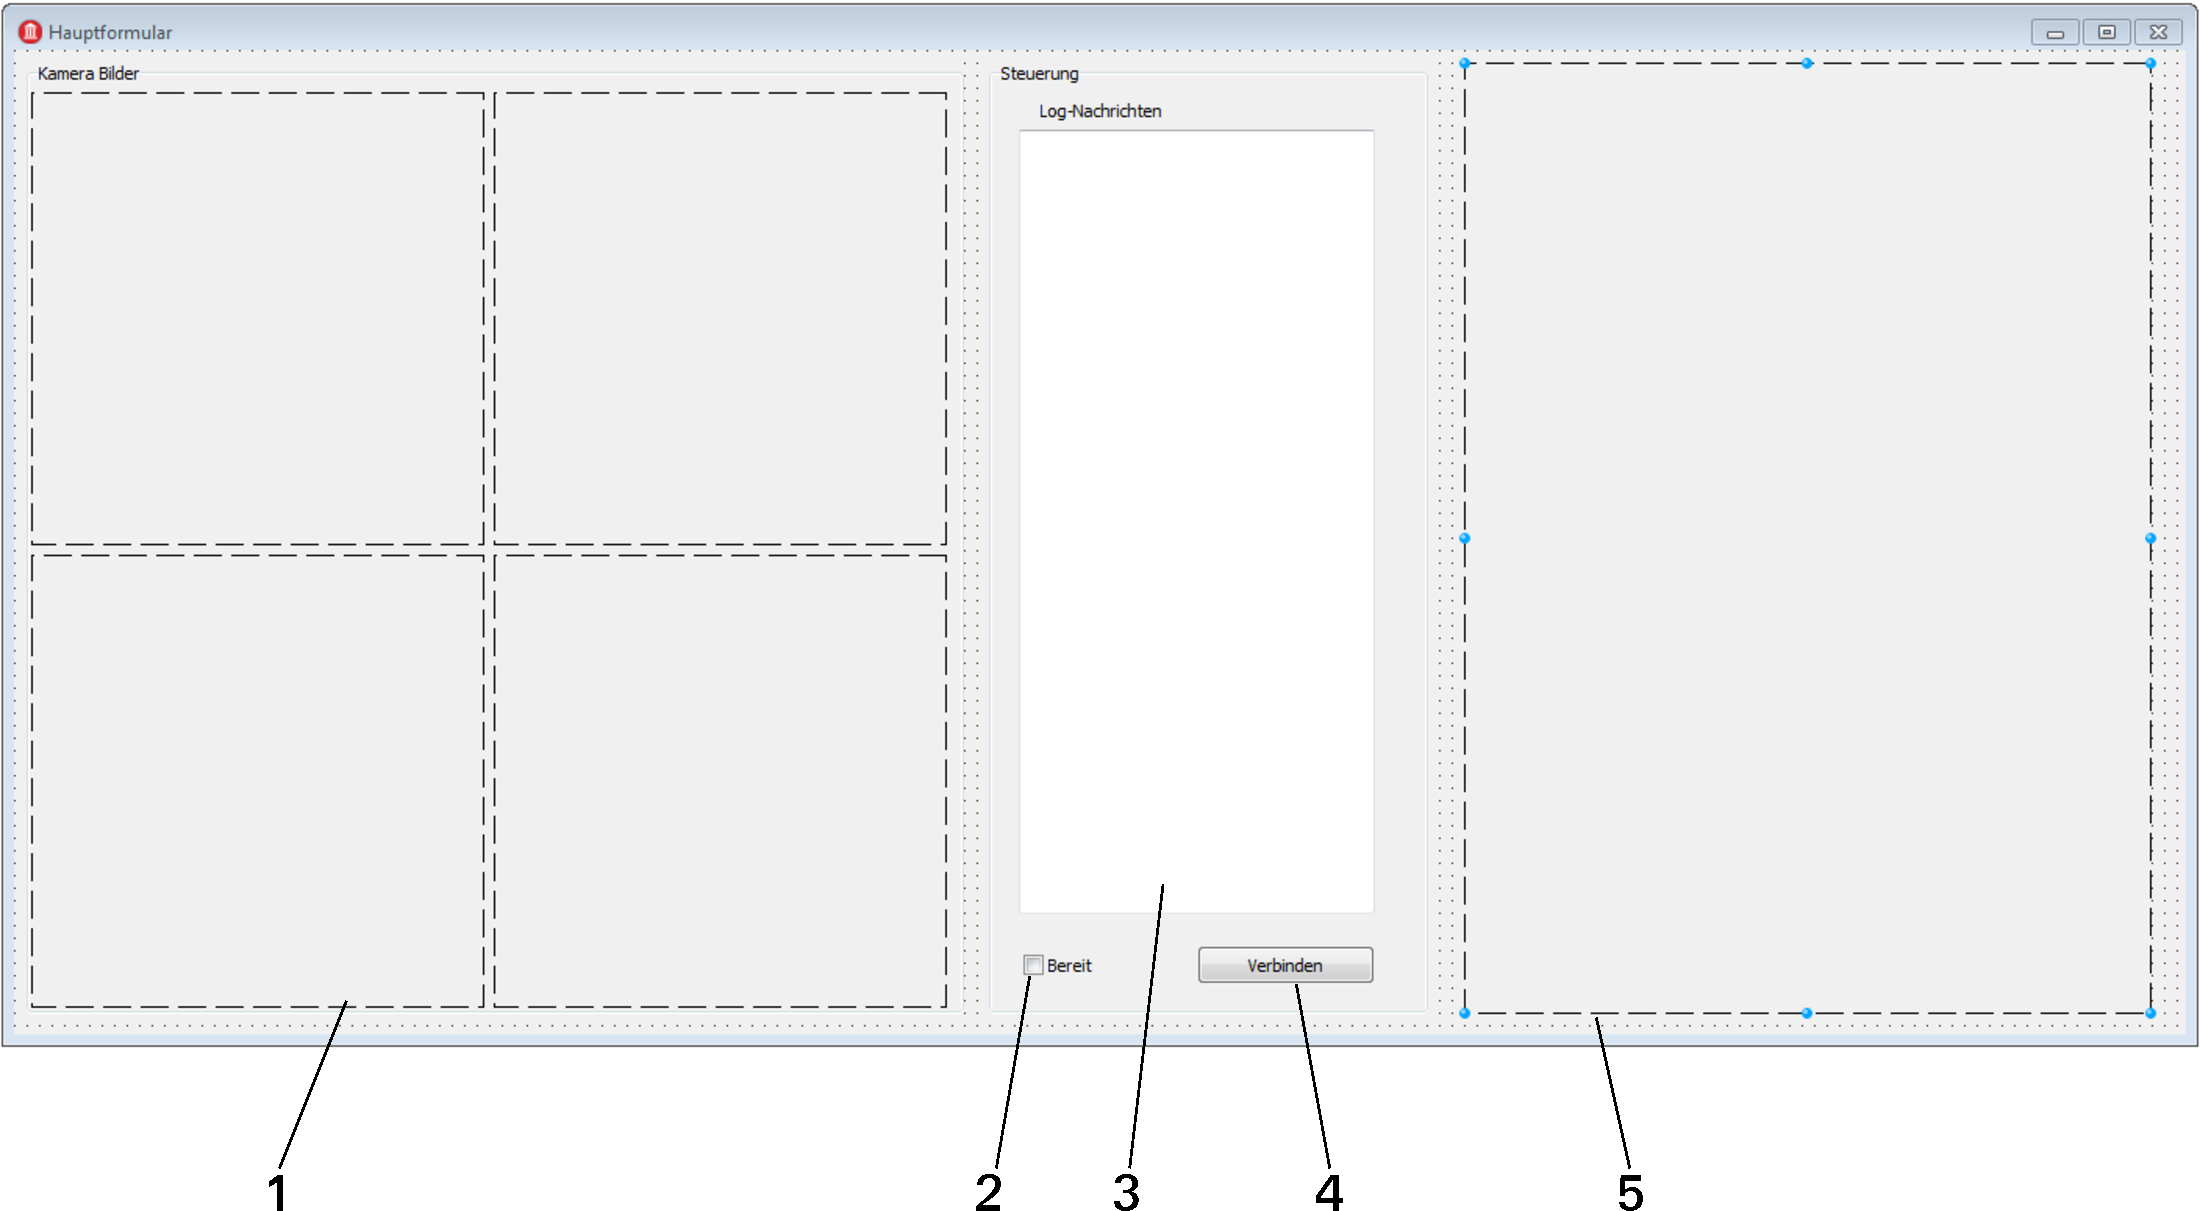
\includegraphics[width=\textwidth]{Bilder/GUI.pdf}
\end{center}
\begin{enumerate}
	\item Anzeige der Bilder, von den USB-Kameras der Roboter 
	\item Kontrollkästchen zum Signalisieren, dass die Roboter bereit sind
	\item Anzeige von Fehler-, Hinweis- und Warnmeldungen
	\item Schaltknopf zum Verbinden der Roboter mit dem Server
	\item Grafische Anzeige der Roboterbewegungen\\
\end{enumerate}
\textbf{Prozeduren:}
\begin{description}
	\item[Ereignisprotokoll] Hinweis-, Fehler- und Warnmeldungen werden in einer Ereignisprotokolldatei abgespeichert, sowie in einem Listenfeld \textbf{"'3"'} angezeigt.
	\item[KamerabilderAnzeigen] Es werden die Bilder der USB-Kameras der Roboter in den Feldern \textbf{"'1"'} angezeigt.
	\item[Visualisierung] In dem Feld \textbf{"'5"'} werden die Bewegungen unserer Roboter grafisch dargestellt.
	\item[FormCreate] In der FormCreate wird das Fenster für das Programm erstellt. Außerdem werden in der FormCreate die IP-Adressen aus einer IP-Config.txt Datei eingelesen und in einem Array abgelegt, dass für die spätere Verbindung zum Server benötigt wird.
\end{description}

\subsection{Klassen}
Für die Berechnungen und Logik haben wir eigene Klassen geschrieben.\\
\newline
Diese unterteilen sich in:
\begin{itemize}
	\item mVektor
	\item mTKI
	\item mKonstanten
	\item mRoboterDaten
\end{itemize}
\subsubsection{mVektor}
Die Klasse mVektor besteht aus dem Record TVektor.
\\
Dieser hat folgende Funktionen, überladende Operatoren und Variablen:
%\newline
%\textbf{Funktionen:}\\
%\newline
%\begin{tabulary}{\textwidth}{|l|l|l|l|}
%	\hline
%	\textbf{Arbeitspaket} & \textbf{AP-Nr.:} & \textbf{Arbeitspaketverantwortlicher} & \bf{Beteiligte Personen}\\
%	\multirow{2}{1cm}{Winkel (überladen)} & 1.1.1 & Sven Stegemann & Eugen Zwetzich\\
%	& & &\\
%	\hline
%	\multicolumn{4}{|l|}{\textbf{Ergebniss:}}\\
%	\multicolumn{4}{|l|}{- Winkel in Bogenmaß}\\
%	\multicolumn{4}{|l|}{}\\
%	\multicolumn{4}{|l|}{\textbf{Aufgabenstellung:}}\\
%	\multicolumn{4}{|p{\textwidth}|}{Es wird der Winkel, zwischen dem Vektor und der X-Achse berechnet und im halboffenen Intervall $[0;2\pi)$ als Bogenmaß zurück gegeben.}\\
%	\hline
%\end{tabulary}
%\\
%\newline
%\\
%\begin{tabulary}{1\linewidth}{|l|l|l|l|}
%	\hline
%	\textbf{Arbeitspaket} & \textbf{AP-Nr.:} & \textbf{Arbeitspaketverantwortlicher} & \bf{Beteiligte Personen}\\
%	\multirow{2}{1cm}{Winkel (überladen)} & 1.1.2 & Sven Stegemann & Eugen Zwetzich\\
%	& & &\\
%	\hline
%	\multicolumn{4}{|l|}{\textbf{Ergebniss:}}\\
%	\multicolumn{4}{|l|}{- Winkel in Bogenmaß}\\
%	\multicolumn{4}{|l|}{}\\
%	\multicolumn{4}{|l|}{\textbf{Aufgabenstellung:}}\\
%	\multicolumn{4}{|p{\textwidth}|}{Es wird der Winkel zwischen zwei Vektoren berechnet und als Bogenmaß zurückgegeben.}\\
%	\hline
%\end{tabulary}
%\\
%\newline
%\\
%\begin{tabulary}{1\linewidth}{|l|l|l|l|}
%	\hline
%	\textbf{Arbeitspaket} & \textbf{AP-Nr.:} & \textbf{Arbeitspaketverantwortlicher} & \bf{Beteiligte Personen}\\
%	Betrag & 1.1.3 & Sven Stegemann & Eugen Zwetzich\\
%	\hline
%	\multicolumn{4}{|l|}{\textbf{Ergebniss:}}\\
%	\multicolumn{4}{|l|}{- Länge des Vektors}\\
%	\multicolumn{4}{|l|}{}\\
%	\multicolumn{4}{|l|}{\textbf{Aufgabenstellung:}}\\
%	\multicolumn{4}{|p{\textwidth}|}{Es wird die euklidische Norm(2-Norm) des Vektors gebildet.}\\
%	\hline
%\end{tabulary}
%\\
%\newline
%\\
%\begin{tabulary}{1\linewidth}{|l|l|l|l|}
%	\hline
%	\textbf{Arbeitspaket} & \textbf{AP-Nr.:} & \textbf{Arbeitspaketverantwortlicher} & \bf{Beteiligte Personen}\\
%	Drehen & 1.1.4 & Sven Stegemann & Michael Mertens\\
%	\hline
%	\multicolumn{4}{|l|}{\textbf{Ergebniss:}}\\
%	\multicolumn{4}{|l|}{- Vektor um Winkel gedreht}\\
%	\multicolumn{4}{|l|}{}\\
%	\multicolumn{4}{|l|}{\textbf{Aufgabenstellung:}}\\
%	\multicolumn{4}{|p{\textwidth}|}{Mit der Drehmatrix wird ein neuer Vektor berechnet, der um einen als Parameter übergebenen Winkel nach links(positiv) bzw. nach rechts(negativ) gedreht ist.}\\
%	\hline
%\end{tabulary}
%\\
%\newline
%\\
%\textbf{Operatoren:}\\
%\newline
%\begin{tabulary}{1\linewidth}{|l|l|l|l|}
%	\hline
%	\textbf{Arbeitspaket} & \textbf{AP-Nr.:} & \textbf{Arbeitspaketverantwortlicher} & \bf{Beteiligte Personen}\\
%	Add & 1.2.1 & Sven Stegemann & Eugen Zwetzich\\
%	\hline
%	\multicolumn{4}{|l|}{\textbf{Ergebniss:}}\\
%	\multicolumn{4}{|l|}{- Summe zweier Vektoren}\\
%	\multicolumn{4}{|l|}{}\\
%	\multicolumn{4}{|l|}{\textbf{Aufgabenstellung:}}\\
%	\multicolumn{4}{|p{\textwidth}|}{Es werden komponentenweise zwei Vektoren addiert und ein neuer Vektor wird zurück gegeben.}\\
%	\hline
%\end{tabulary}
%\\
%\newline
%\\
%\begin{tabulary}{1\linewidth}{|l|l|l|l|}
%	\hline
%	\textbf{Arbeitspaket} & \textbf{AP-Nr.:} & \textbf{Arbeitspaketverantwortlicher} & \bf{Beteiligte Personen}\\
%	Substract & 1.2.2 & Sven Stegemann & Eugen Zwetzich\\
%	\hline
%	\multicolumn{4}{|l|}{\textbf{Ergebniss:}}\\
%	\multicolumn{4}{|l|}{- Differenz zweier Vektoren}\\
%	\multicolumn{4}{|l|}{}\\
%	\multicolumn{4}{|l|}{\textbf{Aufgabenstellung:}}\\
%	\multicolumn{4}{|p{\textwidth}|}{Es werden komponentenweise zwei Vektoren subtrahiert und ein neuer Vektor wird zurück gegeben.}\\
%	\hline
%\end{tabulary}
%\\
%\newline
%\\
%\begin{tabulary}{1\linewidth}{|l|l|l|l|}
%	\hline
%	\textbf{Arbeitspaket} & \textbf{AP-Nr.:} & \textbf{Arbeitspaketverantwortlicher} & \bf{Beteiligte Personen}\\
%	\multirow{2}{1cm}{Multiply (überladen)} & 1.2.3 & Sven Stegemann & Eugen Zwetzich\\
%	& & &\\
%	\hline
%	\multicolumn{4}{|l|}{\textbf{Ergebniss:}}\\
%	\multicolumn{4}{|l|}{- Vektor}\\
%	\multicolumn{4}{|l|}{}\\
%	\multicolumn{4}{|l|}{\textbf{Aufgabenstellung:}}\\
%	\multicolumn{4}{|p{\textwidth}|}{Es werden die einzelnen Komponenten des Vektors mit einem Skalar multipliziert und ein neuer Vektor zurück gegeben.}\\
%	\hline
%\end{tabulary}
%\\
%\newline
%\\
%\begin{tabulary}{1\linewidth}{|l|l|l|l|}
%	\hline
%	\textbf{Arbeitspaket} & \textbf{AP-Nr.:} & \textbf{Arbeitspaketverantwortlicher} & \bf{Beteiligte Personen}\\
%	\multirow{2}{1cm}{Multiply (überladen)} & 1.2.4 & Sven Stegemann & Eugen Zwetzich\\
%	& & &\\
%	\hline
%	\multicolumn{4}{|l|}{\textbf{Ergebniss:}}\\
%	\multicolumn{4}{|l|}{- Skalar}\\
%	\multicolumn{4}{|l|}{}\\
%	\multicolumn{4}{|l|}{\textbf{Aufgabenstellung:}}\\
%	\multicolumn{4}{|p{\textwidth}|}{Es wird ein Skalar mit den einzelnen Komponenten eines Vektors multiplieziert und ein Skalar zurück gegeben.}\\
%	\hline
%\end{tabulary}
%\\
%\newline
%\\
%\begin{tabulary}{1\linewidth}{|l|l|l|l|}
%	\hline
%	\textbf{Arbeitspaket} & \textbf{AP-Nr.:} & \textbf{Arbeitspaketverantwortlicher} & \bf{Beteiligte Personen}\\
%	Equal & 1.2.5 & Sven Stegemann & Eugen Zwetzich\\
%	\hline
%	\multicolumn{4}{|l|}{\textbf{Ergebniss:}}\\
%	\multicolumn{4}{|l|}{- True oder False}\\
%	\multicolumn{4}{|l|}{}\\
%	\multicolumn{4}{|l|}{\textbf{Aufgabenstellung:}}\\
%	\multicolumn{4}{|p{\textwidth}|}{Es wird überprüft ob die Komponenten zweier Vektoren gleich sind.}\\
%	\hline
%\end{tabulary}
%\\
%\newline
%\\
%\textbf{Variablen:}\\
%\newline
%\begin{tabulary}{1\linewidth}{|l|l|l|l|}
%	\hline
%	\textbf{Arbeitspaket} & \textbf{AP-Nr.:} & \textbf{Arbeitspaketverantwortlicher} & \bf{Beteiligte Personen}\\
%	x,y & 1.3.1 & Sven Stegemann & Eugen Zwetzich\\
%	\hline
%	\multicolumn{4}{|l|}{\textbf{Ergebniss:}}\\
%	\multicolumn{4}{|l|}{- }\\
%	\multicolumn{4}{|l|}{}\\
%	\multicolumn{4}{|l|}{\textbf{Aufgabenstellung:}}\\
%	\multicolumn{4}{|p{\textwidth}|}{x, y sind die Komponenten eines Vektors.}\\
%	\hline
%\end{tabulary}

\begin{itemize}
	\item Funktionen
	\begin{description}
		\item[Winkel(überladen)] Berechnet den Winkel zwischen dem Vektor und der X-Achse. Als Rückgabewert erhält man einen Wert im Bogenmaß im Intervall von [0;$2\pi$).
		\item[Winkel(überladen)] Berechnet den Winkel zwischen zwei Vektoren. Als Rückgabewert erhält man einen Wert im Bogenmaß im Intervall von [0;$2\pi$). 
		\item[Betrag] Es wird die Länge des Vektors(euklidische Norm: 2-Norm) berechnet.
		\item[Drehen] Mit der Drehmatrix wird ein neuer Vektor berechnet, der um einen als Parameter übergebenen Winkel nach links(positiv) bzw. nach rechts(negativ) gedreht ist. 
	\end{description}
	\item Operatoren
	\begin{description}
		\item[Add] Es werden die Komponenten der jeweiligen Vektoren addiert und anschließend ein neuer Vektor zurück gegeben.
		\item[Substract] Es werden die Komponenten der jeweiligen Vektoren subtrahiert und anschließend ein neuer Vektor zurück gegeben.
		\item[Multiply(überladen)] Es werden die einzelnen Komponenten des Vektors mit einem Skalar multipliziert und ein neuer Vektor zurück gegeben.
		\item[Multiply(überladen)] Es wird ein Skalar mit den Komponenten eines Vektors multipliziert und ein Skalar zurück gegeben.
		\item[Equal] Es werden die einzelnen Komponenten zweier Vektoren auf Gleichheit überprüft.
	\end{description}
	\item Variablen
	\begin{description}
		\item[x,y] sind die Komponenten eines Vektors.
	\end{description}
\end{itemize}

\subsubsection{mTKI}
Die Klasse mTKI hat einen Datentypen TAktion mit den Werten Fliehen und Fangen und eine abgeleitete Klasse TKI.
\\
Die abgeleitete Klasse TKI besteht aus foglenden Funktionen, Prozeduren und Variablen:\\
\newline
\textbf{Funktionen:}\\
\newline
\begin{tabulary}{1\textwidth}{|l|l|l|l|}
	\hline
	\textbf{Arbeitspaket} & \textbf{AP-Nr.:} & \textbf{Arbeitspaketverantwortlicher} & \bf{Beteiligte Personen}\\
	\multirow{2}{1cm}{Prioritat Festlegen} & 2.1.1 & Sven Stegemann & Eugen Zwetzich\\
	& & &\\
	\hline
	\multicolumn{4}{|l|}{\textbf{Ergebniss:}}\\
	\multicolumn{4}{|l|}{-FLIEHEN}\\
	\multicolumn{4}{|l|}{-FANGEN}\\
	\multicolumn{4}{|l|}{}\\
	\multicolumn{4}{|l|}{\textbf{Aufgabenstellung:}}\\
	\multicolumn{4}{|p{\textwidth}|}{Anhand der Positionsdaten der gegnerischen Roboter wird überprüft, welcher sich am nächsten an unserem Roboter befindet. Anschließend wird über die Winkel Funktion von der Klasse mVektor ermittelt, ob sich dieser Roboter vor oder hinter unserem befindet. Danach wird die Priorität auf FLIEHEN bzw. auf FANGEN gesetzt.}\\
	\hline
\end{tabulary}
\\
\newline
\\
\begin{tabulary}{1\textwidth}{|l|l|l|l|}
	\hline
	\textbf{Arbeitspaket} & \textbf{AP-Nr.:} & \textbf{Arbeitspaketverantwortlicher} & \bf{Beteiligte Personen}\\
	\multirow{2}{1cm}{Fangvektor Berechnen} & 2.1.2 & Sven Stegemann & Jonah Vennemann\\
	& & &\\
	\hline
	\multicolumn{4}{|l|}{\textbf{Ergebniss:}}\\
	\multicolumn{4}{|l|}{-Vektor}\\
	\multicolumn{4}{|l|}{}\\
	\multicolumn{4}{|l|}{\textbf{Aufgabenstellung:}}\\
	\multicolumn{4}{|p{\textwidth}|}{Es wird der Vektor zum nächsten gegnerischen Roboter, der Gefangen werden soll, berechnet. Als Rückgabewert erhält man einen neuen Vektor.}\\
	\hline
\end{tabulary}
\\
\newline
\\
\begin{tabulary}{1\textwidth}{|l|l|l|l|}
	\hline
	\textbf{Arbeitspaket} & \textbf{AP-Nr.:} & \textbf{Arbeitspaketverantwortlicher} & \bf{Beteiligte Personen}\\
	\multirow{2}{1cm}{Fliehvektor Berechnen} & 2.1.3 & Sven Stegemann & Michael Mertens\\
	& & &\\
	\hline
	\multicolumn{4}{|l|}{\textbf{Ergebniss:}}\\
	\multicolumn{4}{|l|}{-Vektor}\\
	\multicolumn{4}{|l|}{}\\
	\multicolumn{4}{|l|}{\textbf{Aufgabenstellung:}}\\
	\multicolumn{4}{|p{\textwidth}|}{Es wird ein Vektor, mit Bezug auf den gegnerischen Roboter von dem Geflohen werden soll, berechnet. Als Rückgabewert erhält man einen neuen Vektor.}\\
	\hline
\end{tabulary}
\\
\newline
\\
\begin{tabulary}{1\textwidth}{|l|l|l|l|}
	\hline
	\textbf{Arbeitspaket} & \textbf{AP-Nr.:} & \textbf{Arbeitspaketverantwortlicher} & \bf{Beteiligte Personen}\\
	\multirow{3}{2cm}{Rand Ausweichvektor Berechnen} & 2.1.4 & Sven Stegemann & Michael Mertens\\
	& & &\\
	& & &\\
	\hline
	\multicolumn{4}{|l|}{\textbf{Ergebniss:}}\\
	\multicolumn{4}{|l|}{-Vektor}\\
	\multicolumn{4}{|l|}{}\\
	\multicolumn{4}{|l|}{\textbf{Aufgabenstellung:}}\\
	\multicolumn{4}{|p{\textwidth}|}{Es wird überprüft ob sich der Roboter im Spielfeld befindet ist dieser außerhalb, so fährt er sofort in's Spielfeld rein. Danach wird überprüft ob sich der Roboter in der Nähe des Spielfeldrandes befindet. Ist dieser zu Nah am Spielfeldrand, wird der Roboter nach links bzw. nach rechts gedreht.}\\
	\hline
\end{tabulary}
\\
\newline
\\
\begin{tabulary}{1\textwidth}{|l|l|l|l|}
	\hline
	\textbf{Arbeitspaket} & \textbf{AP-Nr.:} & \textbf{Arbeitspaketverantwortlicher} & \bf{Beteiligte Personen}\\
	\multirow{4}{2cm}{Roboter Ausweichvektor Berechnen} & 2.1.5 & Sven Stegemann & Michael Mertens\\
	& & &\\
	& & &\\
	& & &\\
	\hline
	\multicolumn{4}{|l|}{\textbf{Ergebniss:}}\\
	\multicolumn{4}{|l|}{-Vektor}\\
	\multicolumn{4}{|l|}{}\\
	\multicolumn{4}{|l|}{\textbf{Aufgabenstellung:}}\\
	\multicolumn{4}{|p{\textwidth}|}{Es wird geprüft welche Roboter aus unserem Team untereinander kollidieren würden. Wurde ein Roboter ermittelt, so wird dieser um die Konstante AUSWEICHWINKEL gedreht. Als Rückgabewert erhält man einen neuen Vektor.}\\
	\hline
\end{tabulary}
\\
\newline
\\
\begin{tabulary}{1\textwidth}{|l|l|l|l|}
	\hline
	\textbf{Arbeitspaket} & \textbf{AP-Nr.:} & \textbf{Arbeitspaketverantwortlicher} & \bf{Beteiligte Personen}\\
	\multirow{2}{1cm}{Rausfahrvektor Berechnen} & 2.1.6 & Sven Stegemann & Michael Mertens\\
	& & &\\
	\hline
	\multicolumn{4}{|l|}{\textbf{Ergebniss:}}\\
	\multicolumn{4}{|l|}{-Vektor}\\
	\multicolumn{4}{|l|}{}\\
	\multicolumn{4}{|l|}{\textbf{Aufgabenstellung:}}\\
	\multicolumn{4}{|p{\textwidth}|}{Sobald ein Roboter als "`Gefangen"' gemeldet ist, wird anhand seiner Position und der Spielfeldgröße ein Vektor zum Herausfahren berechnet. Als Rückgabewert erhält man einen neuen Vektor.}\\
	\hline
\end{tabulary}
\\
\newline
\\
\begin{tabulary}{1\textwidth}{|l|l|l|l|}
	\hline
	\textbf{Arbeitspaket} & \textbf{AP-Nr.:} & \textbf{Arbeitspaketverantwortlicher} & \bf{Beteiligte Personen}\\
	\multirow{2}{1cm}{Serverdaten Empfangen} & 2.1.7 & Sven Stegemann & Michael Mertens\\
	& & &\\
	\hline
	\multicolumn{4}{|l|}{\textbf{Ergebniss:}}\\
	\multicolumn{4}{|l|}{-}\\
	\multicolumn{4}{|l|}{}\\
	\multicolumn{4}{|l|}{\textbf{Aufgabenstellung:}}\\
	\multicolumn{4}{|p{\textwidth}|}{So bald sich der Client mit dem Server verbunden hat, werden die Variablen des Roboters mit Daten vom Server gefüllt.}\\
	\hline
\end{tabulary}
\\
\newline
\\
\begin{tabulary}{1\textwidth}{|l|l|l|l|}
	\hline
	\textbf{Arbeitspaket} & \textbf{AP-Nr.:} & \textbf{Arbeitspaketverantwortlicher} & \bf{Beteiligte Personen}\\
	Anmelden & 2.1.8 & Sven Stegemann & Michael Mertens\\
	\hline
	\multicolumn{4}{|l|}{\textbf{Ergebniss:}}\\
	\multicolumn{4}{|l|}{-}\\
	\multicolumn{4}{|l|}{}\\
	\multicolumn{4}{|l|}{\textbf{Aufgabenstellung:}}\\
	\multicolumn{4}{|p{\textwidth}|}{Ist eine Funktion um sich mit dem Server zu verbinden.}\\
	\hline
\end{tabulary}
\\
\\
\newline
\textbf{Prozeduren:}\\
\newline
\begin{tabulary}{1\textwidth}{|l|l|l|l|}
	\hline
	\textbf{Arbeitspaket} & \textbf{AP-Nr.:} & \textbf{Arbeitspaketverantwortlicher} & \bf{Beteiligte Personen}\\
	\multirow{2}{1cm}{Steuerbefehl Senden} & 2.2.1 & Sven Stegemann & Eugen Zwetzich\\
	& & &\\
	\hline
	\multicolumn{4}{|l|}{\textbf{Ergebniss:}}\\
	\multicolumn{4}{|l|}{-}\\
	\multicolumn{4}{|l|}{}\\
	\multicolumn{4}{|l|}{\textbf{Aufgabenstellung:}}\\
	\multicolumn{4}{|p{\textwidth}|}{Als erstes wird überprüft ob der aktuelle Vektor oder der Zielvektor ein Nullvektor ist. Danach wird ermittelt ob der aktuelle Vektor sich links bzw. rechts vom Roboter befindet. Zum Schluss wird dem Roboter eine Standardgeschwindigkeit übergeben.}\\
	\hline
\end{tabulary}
\\
\newline
\\
\begin{tabulary}{1\textwidth}{|l|l|l|l|}
	\hline
	\textbf{Arbeitspaket} & \textbf{AP-Nr.:} & \textbf{Arbeitspaketverantwortlicher} & \bf{Beteiligte Personen}\\
	\multirow{2}{1cm}{Geschwindigkeit Berechnen} & 2.2.2 & Sven Stegemann & Michael Mertens\\
	& & &\\
	\hline
	\multicolumn{4}{|l|}{\textbf{Ergebniss:}}\\
	\multicolumn{4}{|l|}{-}\\
	\multicolumn{4}{|l|}{}\\
	\multicolumn{4}{|l|}{\textbf{Aufgabenstellung:}}\\
	\multicolumn{4}{|p{\textwidth}|}{Es wird von dem Vektor Geschwindigkeit, die Geschwindigkeit in $\frac{m}{s}$ berechnet.}\\
	\hline
\end{tabulary}
\\
\newline
\\
\begin{tabulary}{1\textwidth}{|l|l|l|l|}
	\hline
	\textbf{Arbeitspaket} & \textbf{AP-Nr.:} & \textbf{Arbeitspaketverantwortlicher} & \bf{Beteiligte Personen}\\
	\multirow{2}{1cm}{Initialisierung} & 2.2.3 & Sven Stegemann & Michael Mertens\\
	& & &\\
	\hline
	\multicolumn{4}{|l|}{\textbf{Ergebniss:}}\\
	\multicolumn{4}{|l|}{-}\\
	\multicolumn{4}{|l|}{}\\
	\multicolumn{4}{|l|}{\textbf{Aufgabenstellung:}}\\
	\multicolumn{4}{|p{\textwidth}|}{Anhand der IP-Adressen, wird jeweils ein Roboter von der Klasse TTXTMobilRoboter erstellt. Ist keine Verbindung möglich, so wird ein Fehler in die Log-Datei geschrieben.}\\
	\hline
\end{tabulary}
\\
\newline
\\
\begin{tabulary}{1\textwidth}{|l|l|l|l|}
	\hline
	\textbf{Arbeitspaket} & \textbf{AP-Nr.:} & \textbf{Arbeitspaketverantwortlicher} & \bf{Beteiligte Personen}\\
	Steuern & 2.2.4 & Sven Stegemann & Michael Mertens\\
	\hline
	\multicolumn{4}{|l|}{\textbf{Ergebniss:}}\\
	\multicolumn{4}{|l|}{-}\\
	\multicolumn{4}{|l|}{}\\
	\multicolumn{4}{|l|}{\textbf{Aufgabenstellung:}}\\
	\multicolumn{4}{|p{\textwidth}|}{Ist eine Funktion um sich mit dem Server zu verbinden.}\\
	\hline
\end{tabulary}

\subsubsection{mKonstanten}
Da wir an verschiedenen Stellen die gleichen Werte benötigten, erstellten wir eine eigene Klasse für Konstanten.
%\newline
%\textbf{Konstanten:}\\
%\newline
%\begin{tabulary}{\textwidth}{|l|l|l|l|}
%	\hline
%	\textbf{Arbeitspaket} & \textbf{AP-Nr.:} & \textbf{Arbeitspaketverantwortlicher} & \bf{Beteiligte Personen}\\
%	Mindestabstand & 3.1.1 & Eugen Zwetzich & Sven Stegemann\\
%	\hline
%	\multicolumn{4}{|l|}{\textbf{Ergebniss:}}\\
%	\multicolumn{4}{|l|}{-}\\
%	\multicolumn{4}{|l|}{}\\
%	\multicolumn{4}{|l|}{\textbf{Aufgabenstellung:}}\\
%	\multicolumn{4}{|p{\textwidth}|}{Ist die Position eines einzelnen Roboters als Vektor.}\\
%	\hline
%\end{tabulary}
%\\
%\newline
%\\
%\begin{tabulary}{\textwidth}{|l|l|l|l|}
%	\hline
%	\textbf{Arbeitspaket} & \textbf{AP-Nr.:} & \textbf{Arbeitspaketverantwortlicher} & \bf{Beteiligte Personen}\\
%	Nullvektor & 3.1.2 & Eugen Zwetzich & Sven Stegemann\\
%	\hline
%	\multicolumn{4}{|l|}{\textbf{Ergebniss:}}\\
%	\multicolumn{4}{|l|}{-}\\
%	\multicolumn{4}{|l|}{}\\
%	\multicolumn{4}{|l|}{\textbf{Aufgabenstellung:}}\\
%	\multicolumn{4}{|p{\textwidth}|}{Ist die Position eines einzelnen Roboters als Vektor.}\\
%	\hline
%\end{tabulary}
%\\
%\newline
%\\
%\begin{tabulary}{\textwidth}{|l|l|l|l|}
%	\hline
%	\textbf{Arbeitspaket} & \textbf{AP-Nr.:} & \textbf{Arbeitspaketverantwortlicher} & \bf{Beteiligte Personen}\\
%	Rand & 3.1.2 & Eugen Zwetzich & Sven Stegemann\\
%	\hline
%	\multicolumn{4}{|l|}{\textbf{Ergebniss:}}\\
%	\multicolumn{4}{|l|}{-}\\
%	\multicolumn{4}{|l|}{}\\
%	\multicolumn{4}{|l|}{\textbf{Aufgabenstellung:}}\\
%	\multicolumn{4}{|p{\textwidth}|}{Ist die Position eines einzelnen Roboters als Vektor.}\\
%	\hline
%\end{tabulary}
%\\
%\newline
%\\
%\begin{tabulary}{\textwidth}{|l|l|l|l|}
%	\hline
%	\textbf{Arbeitspaket} & \textbf{AP-Nr.:} & \textbf{Arbeitspaketverantwortlicher} & \bf{Beteiligte Personen}\\
%	Ausweichwinkel & 3.1.2 & Eugen Zwetzich & Sven Stegemann\\
%	\hline
%	\multicolumn{4}{|l|}{\textbf{Ergebniss:}}\\
%	\multicolumn{4}{|l|}{-}\\
%	\multicolumn{4}{|l|}{}\\
%	\multicolumn{4}{|l|}{\textbf{Aufgabenstellung:}}\\
%	\multicolumn{4}{|p{\textwidth}|}{Ist die Position eines einzelnen Roboters als Vektor.}\\
%	\hline
%\end{tabulary}
%\\
%\newline
%\\
%\begin{tabulary}{\textwidth}{|l|l|l|l|}
%	\hline
%	\textbf{Arbeitspaket} & \textbf{AP-Nr.:} & \textbf{Arbeitspaketverantwortlicher} & \bf{Beteiligte Personen}\\
%	\multirow{2}{1cm}{Länge Fliehvektor} & 3.1.2 & Eugen Zwetzich & Sven Stegemann\\
%	& & &\\
%	\hline
%	\multicolumn{4}{|l|}{\textbf{Ergebniss:}}\\
%	\multicolumn{4}{|l|}{-}\\
%	\multicolumn{4}{|l|}{}\\
%	\multicolumn{4}{|l|}{\textbf{Aufgabenstellung:}}\\
%	\multicolumn{4}{|p{\textwidth}|}{Ist die Position eines einzelnen Roboters als Vektor.}\\
%	\hline
%\end{tabulary}
\begin{itemize}
	\item Variablen
	\begin{itemize}
		\item Mindestabstand
		\item Nullvektor
		\item Rand
		\item Ausweichwinkel
		\item LängeFliehvektor
	\end{itemize}
\end{itemize}

\subsubsection{mRoboterDaten}
Um den Zugriff auf die Daten eines Roboters zu vereinfachen, haben wir diese in einer eigenen Klasse mRoboterDaten untergebracht.
\\
Diese besteht aus einem Record TRoboterDaten mit folgenden Variablen:
\\\\
\textbf{Variablen:}
\begin{itemize}
	\item Position
	\item Geschwindigkeit
	\item Positionsverlauf
	\item Aktiv
\end{itemize}



	\section{Fazit}
In diesem Projekt konnten wir einen guten Einblick in die Planung und die Programmierung eines IT-Projektes erhalten.

Durch die anfängliche Zeitverzögerung bei der Erstellung der Steuerklassen konnten wir nicht wie geplant mit dem Projekt starten, sondern mussten diesen um eine Woche verschieben.

Unter anderem unterschätzten wir am Anfang den Aufwand für die Programmierung der Künstlichen Intelligenz(KI).
Durch diese 2 Probleme mussten wir die anfängliche Planung und das Gantt-Diagramm umstrukturieren.

Der Lernerfolg, den wir durch dieses Projekt erhielten, war sehr groß. Dadurch konnten wir einen praktischen Bezug mit den Vorlesungen in ITPM, Programmiersprachen II und der Mathematik verknüpfen.

Für die Programmierung der Bewegungen bzw. Fahrtrichtungen der Roboter haben wir uns der Vektorrechnung bedient. Diese haben wir in der Mathematik Vorlesung ausführlich kennengelernt und konnten diese für unser Projekt anwenden.

Außerdem konnten wir sehr vieles aus den Vorlesungen bzw. Praktika ITPM und Programmiersprachen II einsetzen.
Z.B. die Kommunikation zwischen den Clients und dem Server mittels dem TCP/IP-Protokoll, Aufwandsschätzung anhand des Function-Point-Verfahrens, sowie die Planung mit Hilfe des Gantt-Charts uvm.
\newpage
	 \definecolor{middlegray}{rgb}{0.5,0.5,0.5}
 \definecolor{lightgray}{rgb}{0.8,0.8,0.8}
 \definecolor{orange}{rgb}{0.8,0.3,0.3}
 \definecolor{yac}{rgb}{0.6,0.6,0.1}

 \lstset{
 	basicstyle=\scriptsize\ttfamily,
 	keywordstyle=\bfseries\ttfamily\color{orange},
 	stringstyle=\color{green}\ttfamily,
 	commentstyle=\color{middlegray}\ttfamily,
 	emph={square}, 
 	emphstyle=\color{blue}\texttt,
 	emph={[2]root,base},
 	emphstyle={[2]\color{yac}\texttt},
 	showstringspaces=false,
 	flexiblecolumns=false,
 	tabsize=2,
 	numbers=left,
 	numberstyle=\tiny,
 	numberblanklines=true,
 	stepnumber=1,
 	numbersep=10pt,
 	xleftmargin=10pt
 }
\newpage
\lstinputlisting[caption={Klasse mTKI}
				 \label{lst:mTKI}, 
				 captionpos=t, language=pascal]
				 {Inhalt/Quellcode/mTKI.pas}
	
\end{document}